\documentclass[conference]{IEEEtran}

% --- REQUIRED PACKAGES ---
\usepackage{amsmath}
\usepackage{amssymb}
\usepackage{graphicx}
\usepackage{booktabs}
\usepackage{url}
\usepackage{bm}

\begin{document}

% --- TITLE & AUTHOR BLOCK ---
\title{Multi Modal Road Assessment}

\author{
\IEEEauthorblockN{Nishkarsh Singhal, Ashutosh Narayan Srivastava, Aryan Yadav, Tushar Basak}
\IEEEauthorblockA{\textit{Electronics and Communication Engineering} \\
\textit{Faculty of Technology, University of Delhi}\\
}
}

\maketitle

% --- ABSTRACT ---
\begin{abstract}
Maintaining high-quality urban road infrastructure is critical for driver safety, vehicle longevity, and efficient city management.
Continuously monitoring road conditions across large urban networks remains a significant logistical challenge: traditional laser profilometry is accurate but prohibitively costly for routine deployment, while existing smartphone-based crowdsensing approaches suffer from static maps, speed-dependent signal artefacts, and no integration with live routing services.
This paper presents a complete, deployed end-to-end system for real-time crowdsourced road surface evaluation, discrete pothole detection, and multimodal navigation.
IRI ground truth is derived from the BeamNG.tech soft-body physics simulator using a five-stage elevation-profile pipeline: (i)~spatial resampling onto a 0.25\,m uniform grid;
(ii)~a curvature-adaptive mesh tessellation correction that suppresses polygon-facet artefacts on curved road geometry while fully preserving roughness on flat sections;
(iii)~the standard 250\,mm ASTM~E1926 tyre-enveloping filter; (iv)~the World Bank Golden Car quarter-car state-space model at 80\,km/h;
and (v)~100\,m segmentation with a 20\,m quarter-car lead-in. The resulting labels train a dual-branch 1D-CNN with an asymmetric Huber loss (4:1 over-prediction penalty) and post-training isotonic regression calibration, achieving a Mean Absolute Error of 1.642\,m/km and $R^{2} = 0.493$ on a held-out test set spanning three vehicle models and three simulated environments.
Complementing the continuous roughness regression, we present a Multimodal Event-Level Pothole Classification model that addresses the distinct detection challenge posed by discrete structural road failures.
The model extracts a Teager-Kaiser Energy Operator (TKEO) spatial signature from the on-road IMU signal to isolate the damped impulse response of the suspension to a pothole contact event.
This kinematic feature is fused with a synchronised dashcam frame via a Physics-Informed Cross-Attention (PICA) layer whose attention weights are explicitly conditioned on vehicle speed and kinetic energy regime, enforcing physical scaling constraints on the multimodal fusion.
A Hunter penalty term within the focal loss prevents false positives from hard-braking events.
The dual-modality system---continuous IRI regression and event-level pothole classification---is unified in a single deployed Android application, backed by a Node.js platform that provides sub-second real-time map updates via Geohash-partitioned WebSocket broadcasting and quality-aware multimodal route planning.
\end{abstract}

% --- KEYWORDS ---
\begin{IEEEkeywords}
International Roughness Index, road surface monitoring, crowdsourcing, smartphone sensing, curvature-adaptive correction, mesh tessellation, 1D convolutional neural network, asymmetric loss, isotonic calibration, multimodal pothole classification, Physics-Informed Cross-Attention, TKEO, event-level anomaly detection, real-time systems, infrastructure-aware routing, ride comfort score, temporal decay, Geohashing, BeamNG simulation.
\end{IEEEkeywords}

% ==========================================
% I. INTRODUCTION
% ==========================================
\section{Introduction}

\subsection{The Global Road Deterioration Problem}
Road pavement is the most capital-intensive component of urban infrastructure.
In India alone, the road network spans over 6.3 million kilometres [1], yet a large fraction of this network---particularly secondary and tertiary roads---receives structural condition assessment no more frequently than once every three to five years, if at all [1].
The World Bank estimates that the cumulative economic cost of poor road condition to vehicle owners exceeds \$500 billion annually worldwide, through accelerated tyre wear, fuel overconsumption, drivetrain damage, and road accident costs attributable to surface defects [2].
At the extremes of the spectrum, potholes---full-depth structural failures caused by the interaction of water infiltration, traffic loading, and thermal cycling---are responsible for thousands of vehicle damage incidents and road accidents annually, and their formation can progress from surface cracking to a full pothole within a matter of weeks under heavy precipitation.
The international standard for quantifying road roughness is the International Roughness Index (IRI), defined by the World Bank Quarter-Car model and standardised in ISO 8608 and ASTM E1926 [3].
IRI represents the cumulative vertical displacement of a standardised quarter-car suspension traversing a road at 80 km/h, expressed in metres per kilometre ($\text{m/km}$).
Professional measurement uses inertial laser profilometry vehicles whose procurement and operational costs are prohibitive for routine city-scale deployment.
This creates a fundamental monitoring gap: the condition of the road network degrades continuously between surveys, and defects go unreported for months.
The challenge of closing this monitoring gap---with high spatial resolution, at low cost, and in near-real-time---motivates this work.

\subsection{The Smartphone Sensing Opportunity}
Every smartphone in use today is a capable mobile sensor platform: it contains a multi-axis MEMS inertial measurement unit (IMU), a GNSS receiver, and a persistent mobile data connection.
With over 6.8 billion smartphones in global use, any vehicle in which a smartphone is mounted constitutes a potential road condition probe.
If even a small fraction of the daily vehicle trips on a road network contribute passive IMU measurements, the aggregate creates a continuously updated, spatially dense picture of road condition at near-zero marginal cost---a paradigm known as participatory or opportunistic sensing [4].
This vision has motivated a growing body of research since Mohan et al.'s foundational Nericell system (2008) [5].
However, despite more than fifteen years of effort, no existing system achieves the full promise of this paradigm.
Three fundamental limitations persistently appear across the literature and remain unresolved.

\subsection{Three Unsolved Limitations of the State of the Art}

\textbf{Limitation 1 --- Speed-Dependent Signal Distortion and the Staircase Artifact:} IMU sensors produce measurements as a function of time.
Road roughness, however, is a geometric property of a spatial surface.
The relationship between the two is mediated by vehicle speed $v$: a surface undulation of spatial wavelength $\lambda$ (metres) produces a temporal frequency $f = v / \lambda$ in the IMU signal.
This means that the same physical road feature appears at different temporal frequencies at different speeds.
At $v = 10~\text{km/h}$, a 5-metre undulation appears at $\approx 0.56~\text{Hz}$;
at $v = 50~\text{km/h}$, the same feature appears at $\approx 2.78~\text{Hz}$---a five-fold shift.
Any time-domain filter or time-domain machine learning model (including convolutional neural networks applied to raw IMU time series) is therefore inherently speed-dependent.
The practical consequence is the ``staircase artifact'': at locations where vehicle speed changes abruptly---intersections, pedestrian crossings, traffic lights, roundabouts---time-domain processing pipelines produce discontinuous, step-change jumps in estimated road quality even on physically uniform surfaces.
This is because the pipeline's effective spatial frequency resolution changes with speed, and the transition appears as a sudden change in the measured roughness signal.
Mukherjee et al. [6] acknowledge speed as a confounding factor and apply post-hoc normalisation; Sattar et al.
[7] restrict experiments to highway driving at near-constant speed; the comprehensive review by the MDPI 2024 survey [8] identifies speed variation as one of the two primary open challenges in the field.
No prior system has structurally eliminated this artifact through a full spatial-domain signal processing pipeline.

\textbf{Limitation 2 --- No Temporal Road State Evolution (The Stale Map Problem):} A road is not a static object.
Its condition evolves continuously: a pothole that appears in February after winter frost-damage may be repaired by the municipal authority in March.
A smooth surface may develop cracking by summer under heavy truck traffic.
Any crowdsourced road condition map must model this temporal evolution---otherwise, the map becomes progressively stale and misleading.
Repaired sections must eventually transition back to baseline.
Once a defect observation is stored, it persists indefinitely. Citizen reporting platforms such as SeeClickFix and FixMyStreet require explicit administrator action to close a report [9].
Academic systems including iDriveSense [10] and Roadroid [11] store observations without temporal weighting.
Waze's pothole reporting, evaluated by Goodall (2023) [9], clears reports after 30 minutes unless confirmed---a heuristic that bears no relationship to the actual timescale of road repair.
The result is that in all prior systems, a road repaired today will still show as damaged on the map for an indeterminate period, severely degrading user trust and map utility.

\textbf{Limitation 3 --- Absence of End-to-End Multimodal Navigation Integration:} The ultimate utility of a road condition sensing system is not just awareness---it is the ability to act on that awareness.
A driver who knows that Route A has a pothole cluster 2 km ahead should be able to choose Route B, with full knowledge of the trade-off between the extra distance and the improved ride quality.
This is the multi-criteria route planning problem: finding a route that optimises a composite objective of travel distance, travel time, and infrastructure quality.
Despite this obvious utility, no existing peer-reviewed system delivers a complete, live, navigation-integrated deployment in which road quality derived from crowdsourced smartphone sensing is used as a first-class routing criterion.
iDriveSense [10] proposes a fuzzy-logic route scoring mechanism but relies on manually annotated road quality maps rather than a continuously updated crowdsourced layer, and is not deployed as a working mobile application.
The system of Dewangan et al. [12] and the pothole avoidance framework of Balakuntala et al.
[13] are conceptual frameworks without real-time backend integration. Commercial navigation systems (Google Maps, HERE, Waze) do not incorporate independently computed IRI-based quality scores.
This gap---between a working crowdsourced sensing backend and a real, multimodal navigation experience for the end user---represents the most practically impactful limitation in the field.

\subsection{Additional Gaps in Prior Work}
Beyond the three primary limitations, a systematic review of the literature reveals several weaknesses:

\textbf{Vehicle-Suspension Coupling and the Cross-Vehicle Generalisation Problem:} Virtually all empirical training datasets are collected from a single vehicle or a small number of homogeneous vehicles.
The suspension system of a rigid heavy vehicle filters road surface inputs very differently from a soft-sprung passenger car: the same road profile produces different IMU signal amplitudes, damping profiles, and resonant frequencies across vehicle classes.
A model trained on data from one vehicle type and deployed on another exhibits systematic, uncorrected bias [6], [7].
Only a handful of works attempt cross-vehicle normalisation, and none solve the problem from first principles.

\textbf{Absence of Physically Calibrated Ground Truth:} The majority of published systems label their training data with subjective human ratings (good/fair/poor), manual event annotations, or binary thresholds on the z-axis accelerometer [14], [11].
These labels are not reproducible, not physically calibrated, and not inter-comparable across studies.
The IRI is the internationally standardised metric of road roughness [3], but obtaining true IRI ground truth in the field requires co-registered laser profilometry---a logistical challenge that most papers do not address.
This absence of calibrated ground truth makes rigorous comparison between published systems impossible.

\textbf{Computational Deployability:} Systems that achieve high detection accuracy often do so at the cost of models too large or computationally expensive for continuous background inference on a smartphone [8].
Large LSTM networks, multi-scale ResNets, and attention-based transformers may achieve strong performance on server-side batch evaluation but are impractical as always-on on-device sensors due to battery and thermal constraints.

\textbf{No Personal Ride History or Longitudinal Comfort Analytics:} No existing system maintains a per-user ride history that allows individuals to understand their cumulative road experience over time---which routes they regularly travel, how the quality of those routes has evolved, and what their average Ride Comfort Score is.
This longitudinal dimension is entirely absent from the academic literature, despite its obvious value for urban mobility analytics and municipal reporting.

\subsection{Contributions of This Paper}
This paper presents a complete, deployed, end-to-end system for real-time crowdsourced road surface evaluation and multimodal navigation.
Our specific contributions, each addressing one of the gaps identified above, are as follows:

\begin{enumerate}
    \item \textbf{Curvature-adaptive mesh tessellation correction for simulator-derived IRI:} We identify and resolve a systematic polygon-facet reporting bias in BeamNG.tech elevation profiles that inflates calculated IRI to 15--16\,m/km on geometrically smooth ramps and flyovers.
Our correction blends a 5\,m moving-average profile using a curvature-dependent weight $\alpha = \text{clip}\bigl((\kappa - \kappa_{\text{thresh}}) / 5\kappa_{\text{thresh}},\, 0,\, 1\bigr)$, leaving flat sections entirely untouched ($\kappa < \kappa_{\text{thresh}}$, $\alpha \approx 0$) while suppressing mesh facet artefacts on curved geometry.
This enables physically valid IRI ground truth to be generated across all road geometries present in the simulator.

    \item \textbf{Physics-simulation-derived, vehicle-agnostic IRI ground truth via BeamNG.tech:} We exploit the BeamNG.tech soft-body physics simulator---the same platform used for ADAS research and autonomous driving validation~\cite{15}---to generate synchronised IMU and elevation-profile data pairs across multiple vehicle models driving at highly variable speeds.
Elevation profiles acquired by downward-facing LiDAR sensors are processed through a five-stage pipeline (spatial resampling, curvature-adaptive correction, 250\,mm tyre-enveloping filter, Golden Car quarter-car model at the standardised 80\,km/h, 100\,m segmentation) to yield calibrated \texttt{readings\_2.csv} IRI labels that cannot be practically obtained from field surveys.

    \item \textbf{Dual-branch 1D-CNN with asymmetric loss and isotonic calibration:} We propose a compact dual-branch network combining depthwise-separable 1D convolutions over 100\,m IMU windows with a dense context branch processing mean speed, mean $a_z$, and zero-crossing rate.
Vertical acceleration is normalised by $(22.22/v_{\text{safe}})^2$ to account for velocity-squared suspension scaling, rendering the feature vehicle-speed-agnostic.
An AsymmetricHuberLoss ($\delta=1.0$, 4:1 over-prediction penalty) addresses the under-prediction failure mode on high-IRI roads, and post-training isotonic regression calibration further corrects systematic bias.
Deployed via TensorFlow Lite ($\approx$41.4\,KB, $<$5\,ms), the model achieves MAE 1.642\,m/km and $R^{2} = 0.493$ on held-out trips.

    \item \textbf{Multimodal Event-Level Pothole Detection with Physics-Informed Cross-Attention:} We present a fusion architecture for discrete pothole detection that combines the Teager-Kaiser Energy Operator (TKEO) spatial kinematic signature $S(d)$---which amplifies the damped impulse response of the suspension to a structural road failure---with synchronised dashcam imagery via a Physics-Informed Cross-Attention (PICA) layer.
Attention weights are conditioned on vehicle speed and kinetic energy regime, enforcing physical scaling constraints on the multimodal fusion.
A Hunter penalty term within the focal loss explicitly suppresses false positives from hard-braking events, whose IMU signature would otherwise be indistinguishable from genuine pothole contacts.

    \item \textbf{Temporally adaptive crowdsourced map with self-healing consistency:} We implement an exponential time-decay aggregation model ($w \propto e^{-t/\tau}$) in which every observation's contribution to a road segment's quality score diminishes with age.
This enables repaired road defects to be automatically and continuously down-weighted without any manual intervention---a property we term \textit{self-healing map consistency}, not previously described in the literature.

    \item \textbf{Sub-second real-time broadcast via Geohash WebSocket namespacing:} The distributed backend routes road quality events exclusively to clients whose geographic viewport overlaps the affected area, using precision-6 Geohash strings as Socket.IO room identifiers.
This achieves O(R) broadcast complexity ($R =$ clients in a $\approx 1.2~\text{km} \times 0.61~\text{km}$ cell) without global broadcast overhead.

    \item \textbf{Multimodal ride-comfort-aware routing:} A routing service retrieves multiple candidate routes from the Mapbox Directions API, scores each by a distance-weighted composite of IRI-based road quality and route length, and presents the user with a ranked multi-route comparison.
Users can select their preferred balance between ride comfort and distance---directly addressing the multi-criteria route planning gap identified above.

    \item \textbf{Personal Ride Comfort Score and trip history:} Each completed journey is stored as a user-associated record containing the route geometry, mean IRI, and an overall Ride Comfort Score derived from the spatial quality distribution of the traversed road.
This enables longitudinal personal mobility analytics and provides municipalities with user-linked pavement condition reports.
\end{enumerate}

\subsection{Paper Organisation}
Section :: surveys related work across road surface monitoring, crowdsourcing architectures, and infrastructure-aware routing.
Section ::: details the complete methodology and system architecture. Section IV presents experimental results.
Section V discusses current limitations and future work---including the Pothole Classification Model under active development. Section VI concludes.

% ==========================================
% II. RELATED WORK
% ==========================================
\section{Related Work}

\subsection{Traditional Road Condition Assessment}
The established method for road condition assessment is the inertial laser profilometer: a vehicle-mounted system that uses laser displacement sensors and a high-precision IMU to measure the road surface profile at driving speeds of 60--100 km/h, computing IRI in accordance with ASTM E1926.
These systems achieve high accuracy (IRI precision $\pm0.1~\text{m/km}$) but cost upward of \$200,000 USD per vehicle, require skilled operators, and are logistically suited only to periodic surveys---not continuous monitoring.
Some agencies use Response Type Road Roughness Measurement Systems (RTRRMS), such as bump integrators mounted in standardised vehicles, which are cheaper but provide lower accuracy and require correlation calibration.
Ground-penetrating radar, 3D LiDAR scanning, and photogrammetric inspection from unmanned aerial vehicles (UAVs) have been proposed for crack detection and structural assessment;
these methods provide rich surface geometry but at high per-km cost and low temporal frequency, making city-scale continuous monitoring impractical.

\subsection{Simulator-Based IRI Ground Truth and Mesh Tessellation Artefacts}
The logistical difficulty of co-registering laser-profilometer IRI measurements with synchronised IMU recordings across multiple vehicle types has prompted a growing interest in physics-simulation-based data generation.
BeamNG.tech~\cite{15} offers a soft-body finite-element vehicle model whose tyre--road interaction fidelity is sufficient for ADAS and autonomous-driving research, providing oracle access to both vehicle kinematics and road surface geometry within a single deterministic environment.
A non-obvious complication specific to polygon-mesh simulators is the \textbf{mesh tessellation artefact}: road surfaces are rendered from planar polygon facets.
On flat roads the facets are imperceptible; on sections with vertical curvature---flyovers, ramps, and grade transitions---adjacent facets meet at small dihedral angles, producing a systematic high-frequency oscillation in the sampled elevation profile.
This oscillation is a geometric rendering distortion rather than physical road roughness: on a geometrically smooth ramp its spatial frequency falls in the same band (1--3\,m wavelength) that the Quarter-Car model is most sensitive to, causing raw IRI values to inflate to 15--16\,m/km on surfaces that are, by design, perfectly smooth.
This artefact has not been previously identified or corrected in the literature on simulator-based road sensing datasets.
Our curvature-adaptive tessellation correction (Section~\ref{sec:iri_pipeline}) directly addresses this gap.

% ==========================================
% III. METHODOLOGY AND SYSTEM ARCHITECTURE
% ==========================================
\section{Methodology and System Architecture}

\begin{figure*}[t]
    \centering
    
\includegraphics[width=\textwidth]{images/system_architecture.png}
    \caption{Complete system architecture for sensor data acquisition, ground truth generation, and machine learning inference.
\textit{Left}: the BeamNG.tech simulation environment providing four synchronised data acquisition modules (road geometry via LiDAR, elevation profile, IMU and vehicle dynamics, and dashcam imagery), followed by the spatial resampling and synchronisation pipeline.
\textit{Top right (blue)}: the Continuous IRI Estimation Pipeline---the ground truth flow (raw elevation $\to$ curvature-adaptive mesh tessellation correction $\to$ 250\,mm tyre-enveloping filter $\to$ Golden Car quarter-car simulation at 80\,km/h) and the predictive model flow (raw IMU $\to$ spatial resampling and speed normalisation $\to$ dual-branch 1D-CNN with DepthwiseConv1D, dual global pooling, and context statistics extractor $\to$ feature fusion $\to$ regression head with asymmetric Huber loss).
\textit{Bottom right (orange)}: the Multimodal Road Anomaly Classification Pipeline---kinematic pathway (TKEO processing $\to$ spatial signature generation $\to$ kinematic encoder), vision pathway (dashcam imagery $\to$ vision encoder), and context pathway (vehicle speed and kinetic energy regime), fused via a Physics-Informed Cross-Attention (PICA) module and trained with focal loss and the Hunter penalty for braking-artefact suppression.}
    \label{fig:system_architecture}
\end{figure*}

\subsection{Synthetic Data Acquisition and Ground Truth Generation}

\subsubsection{The Fundamental Problem with Empirical Datasets}
A recurring limitation in prior smartphone-based road profiling literature is the reliance on empirical, field-collected datasets for model training and ground truth establishment.
While seemingly natural, this approach introduces a profound and often underappreciated confound: \textbf{the physical coupling between the road surface and the IMU sensor is not fixed.} It is mediated by the vehicle's suspension system---a highly nonlinear, vehicle-specific, and load-dependent mechanical transfer function.

Formally, if we denote the true road profile as $h(x)$ and the sensor-observed vertical acceleration as $a_z(t)$, the empirical relationship is:

\begin{equation}
\begin{split}
a_z(t) &= \mathcal{T}_{\text{veh}}(h(x(t)), \dot{x}(t), m_{\text{load}}, T_{\text{ambient}}) \\
&\quad + \epsilon(t)
\end{split}
\end{equation}

where $\mathcal{T}_{\text{veh}}$ is an unknown, nonlinear operator characterizing the vehicle's full suspension dynamics, $\dot{x}(t)$ is the instantaneous speed, $m_{\text{load}}$ is the payload mass, $T_{\text{ambient}}$ is the ambient temperature (which affects tire pressure 
and damper viscosity), and $\epsilon(t)$ is sensor noise. This operator is not only \textbf{unknown} for any given vehicle but is \textbf{different across vehicles.} A model trained on a dataset collected in a mid-size sedan will exhibit systematic bias when deployed on a utility vehicle with stiffer suspension---even on identical roads---because $\mathcal{T}_{\text{veh}}$ differs fundamentally between the two platforms.
Furthermore, empirical field collection makes it practically impossible to obtain a true, decoupled ground truth for $h(x)$.
Laser profilometers or road-and-level instruments can provide such ground truth, but co-registering their spatial measurements with the corresponding IMU time series across diverse road conditions, vehicle speeds, and vehicle types is logistically intractable at the scale required to train a robust deep learning model.
This paper directly resolves both problems through the use of a physics simulation environment.

\subsubsection{The BeamNG.tech Soft-Body Physics Engine as a Deterministic Laboratory}
We employ \textbf{BeamNG.tech} (v0.38.3.0), a professional-grade vehicular dynamics simulator based on a soft-body physics model, as our synthetic data generation environment.
This is a fundamental departure from prior work. The simulation's physical fidelity is sufficient for automotive engineering research precisely because it models vehicles not as rigid bodies with simplified spring-damper suspension proxies, but as fully deformable finite-element meshes where every node participates in the physical simulation.
The tire-road interaction, damper hysteresis, and chassis flex are all modeled from first principles.
The critical advantage of this approach is \textbf{Oracle Access to Ground Truth.} Within the simulation, we have simultaneous, synchronized, zero-noise access to:
\begin{enumerate}
    \item \textbf{The true road surface geometry} $h(x)$, obtained directly via dual downward-facing LiDAR sensors mounted at the left and right wheel tracks, whose output is logged to \texttt{iri\_sensor\_data.csv}.
    \item \textbf{The vehicle-filtered IMU response} $(a_x, a_y, a_z, \omega_x, \omega_y, \omega_z)$ and vehicle speed, obtained from a virtual \texttt{AdvancedIMU} sensor positioned at the vehicle dashboard---precisely replicating a smartphone in a dashboard mount---and logged to \texttt{imu\_speed\_data.csv}.
    \item \textbf{The vehicle's true kinematic state}, including instantaneous 2D position $(p_x, p_y)$ used for cumulative horizontal distance computation in the IRI pipeline.
\end{enumerate}

The code reflects this three-thread architecture explicitly. A \texttt{bng\_lock} serializes all communication with the physics engine, while a \texttt{data\_lock} protects the \texttt{shared\_data} dictionary that is written by sensor worker threads and consumed by the main logging loop.
Three daemon threads run in parallel:
\begin{itemize}
    \item \textbf{\texttt{ImuStateWorker}}: Polls the virtual \texttt{AdvancedIMU} sensor and vehicle state at $f_{\text{IMU}} = 100~\text{Hz}$, extracting and re-mapping acceleration and angular velocity axes to match real-world smartphone conventions (BeamNG's native coordinate system differs from the standard right-hand IMU frame).
Writes IMU channels, speed, and position to \texttt{imu\_speed\_data.csv}.
    \item \textbf{\texttt{LidarWorker}}: Polls two narrow-beam downward-facing LiDAR sensors (mounted at $\pm 0.85~\text{m}$ lateral offset, approximating wheel-track positions) at $f_{\text{IRI}} = 100~\text{Hz}$, extracting the mean Z-elevation of the point cloud to yield instantaneous road surface height $h_L(t)$ and $h_R(t)$.
Writes elevation channels and position to \texttt{iri\_sensor\_data.csv}.
    \item \textbf{\texttt{CameraWorker}}: Captures a forward-facing dashcam view at $f_{\text{CAM}} = 20~\text{Hz}$ for qualitative inspection and pothole classification.
\end{itemize}

The critical coordinate re-mapping performed in \texttt{ImuStateWorker} deserves explicit documentation, as it is an often-silently-introduced source of error in simulation-to-real transfer:

\begin{table}[htbp]
\centering
\caption{Coordinate Re-mapping from BeamNG to Physical IMU Frame}
\label{tab:imu_mapping}
\resizebox{\columnwidth}{!}{
\begin{tabular}{lll}
\toprule
\textbf{BeamNG Raw Channel} & \textbf{Physical Axis} & \textbf{Mapped Key} \\
\midrule
\texttt{acc[2]} (Lateral, Y-world) & Left-Right & \texttt{ax} \\
\texttt{acc[0]} (Longitudinal, X-world) & Front-Back & \texttt{ay} \\
\texttt{acc[1]} (Vertical, Z-world) & Up-Down & \texttt{az} \\
\texttt{gyro[2]} (Pitch rate) & Around X-lateral & \texttt{wx} \\
\texttt{gyro[0]} (Roll rate) & Around Y-longitudinal & \texttt{wy} \\
\texttt{gyro[1]} (Yaw rate) & Around Z-vertical & \texttt{wz} \\
\bottomrule
\end{tabular}
}
\end{table}

The main logging loop runs as a \textbf{strict metronome} using \texttt{time.perf\_counter()}, enforcing a precisely $\Delta t = 10~\text{ms}$ cadence 
between samples, independent of any individual sensor's polling latency. This ensures both CSV logs have uniform temporal spacing---a prerequisite for the IRI computation pipeline described in Section~\ref{sec:iri_pipeline}.

\begin{figure*}[t]
    \centering
    
\includegraphics[width=0.8\textwidth]{images/iri/beamNG_sensor_placement.jpg}
    \caption{Sensor placement and spatial sampling architecture within the BeamNG.tech simulation environment.}
    \label{fig:sensor_placement}
\end{figure*}

A critical design decision in the data collection protocol concerns vehicle speed.
A naive approach would simulate all vehicles driving at a constant $v = 80~\text{km/h}$---the ISO~8608 standardised speed for IRI computation---throughout every run.
This would, however, introduce a severe speed-overfitting bias into the learned model: the 1D-CNN would learn correlations between the specific IMU frequency signatures produced at 80\,km/h and the IRI label, and would fail to generalise to real-world deployment conditions where vehicle speed varies continuously with traffic, road geometry, and driver behaviour.
To mitigate this, vehicles were instead simulated at \textbf{highly variable speeds}, deliberately capturing the full spectrum of real urban driving: rash driving at high speed on open stretches, careful slow driving in congested zones, and normal mixed-traffic conditions.
This variable-speed protocol ensures that the IMU signal space seen by the model spans the full range of operational conditions, preventing the network from learning any speed-specific shortcut.
The resulting time-domain IMU records contain diverse speed signatures that the model must learn to discount, retaining only the road-profile-dependent components.
Critically, this speed variability affects only the \textbf{IMU feature data}, not the IRI ground truth label.
The IRI is a property of the road surface geometry $h(x)$, not of any particular traversal speed.
After collecting the elevation profile $h_L(l)$ and $h_R(l)$ via spatial resampling (Section~\ref{sec:iri_pipeline}), the Golden Car quarter-car state-space model is run over this spatial profile at the standardised $v_{\text{ref}} = 80~\text{km/h}$ (22.22\,m/s) to generate the IRI ground truth, irrespective of the actual speed at which the vehicle traversed the road during data collection.
This decoupling of the IMU feature collection (variable speed) from the IRI label generation (fixed reference speed) is the key methodological property that enables the model to learn a speed-invariant mapping from IMU response to road roughness.
We collect data across three distinct virtual maps---\texttt{east\_coast\_usa} (hilly terrain with unpaved sections), \texttt{automation\_test\_track} (controlled circuit with varied surface types), and \texttt{west\_coast\_usa} (highway and urban arterials)---and across three vehicle models (\texttt{hopper}, \texttt{sunburst2}, \texttt{vivace}) representing a range of suspension stiffnesses.
This multi-vehicle, multi-environment corpus ensures that the learned model generalises across both the suspension-coupling variability and the speed-profile diversity that plague empirical approaches.

% ---------------------------------------------------------
\subsection{IRI Computation Pipeline}
\label{sec:iri_pipeline}

The two CSV files produced by the data acquisition stage---\texttt{imu\_speed\_data.csv} (IMU channels, speed, position) and \texttt{iri\_sensor\_data.csv} (left and right road surface elevation, position)---are processed by \texttt{iri\_calculation.py} to yield the labelled dataset \texttt{readings\_2.csv}.
The pipeline comprises five steps.

\subsubsection{Step 1: Spatial Resampling}

After merging the two CSVs on \texttt{sample\_number} and \texttt{sim\_time}, the cumulative 2D horizontal distance is computed from successive position deltas:

\begin{equation}
\label{eq:cum_dist}
l_k = \sum_{i=1}^{k} \sqrt{(\Delta p_{x,i})^2 + (\Delta p_{y,i})^2}
\end{equation}

The 2D projection is used because the IRI standard is defined for the along-road distance profile;
using horizontal distance rather than 3D arc-length avoids conflating road slope with roughness.
The left and right elevation profiles $h_L(l)$ and $h_R(l)$ are then linearly interpolated onto a uniform spatial grid with spacing $\Delta x = 0.25\,\text{m}$---the canonical sample interval specified in WB TP46 and ASTM~E1926~\cite{sayers1986guidelines}.

\subsubsection{Step 2: Curvature-Adaptive Mesh Tessellation Correction}

BeamNG.tech renders road surfaces from planar polygon meshes. On flat sections these facets are imperceptible;
however, on segments with vertical curvature---flyovers, ramps, and grade transitions---adjacent facets meet at small dihedral angles, producing a systematic high-frequency oscillation in the sampled elevation profile even on geometrically smooth slopes.
Left uncorrected, this distortion inflates the computed IRI to 15--16\,m/km on surfaces that are, by construction, smooth.
This is a data-quality issue specific to polygon-mesh simulators, not a reflection of real road roughness.

Figure~\ref{fig:mesh_psd} provides direct empirical evidence of this phenomenon. The left column shows a representative \textit{flat} section: the elevation profile is smooth, the slope signal is essentially zero-mean with low-amplitude noise, and the Power Spectral Density (PSD) of the slope shows negligible energy in the IRI-sensitive wavelength band (1--30\,m, shaded).
The right column shows the \textit{steepest} section in the same dataset: the elevation profile rises monotonically, yet the slope signal exhibits violent high-frequency oscillations with peak-to-peak amplitude of $\pm 0.3$\,m/m---four to five times larger than any real road roughness---and the PSD confirms that these oscillations are concentrated precisely in the 1--10\,m wavelength band, the band to which the Golden Car quarter-car model is most sensitive.
These oscillations are polygon-facet jitter: a pure geometric rendering distortion of the mesh that vanishes on flat terrain and becomes severe wherever the road has non-zero vertical curvature.

\begin{figure*}[t]
    \centering
    
\includegraphics[width=\textwidth]{images/iri/mesh_poygon_analysis.png}
    \caption{Empirical evidence of polygon-mesh tessellation jitter in BeamNG.tech simulation data.
\textit{Left column}: flattest road section---smooth elevation profile, low-amplitude slope noise, and negligible PSD energy in the IRI-sensitive wavelength band (shaded).
\textit{Right column}: steepest road section---monotonically rising elevation, but severe high-frequency slope oscillations ($\pm 0.3$\,m/m peak-to-peak) whose PSD is concentrated entirely in the 1--10\,m IRI-sensitive band.
This jitter is a geometric rendering distortion of planar polygon facets meeting at dihedral angles on curved geometry;
it does not exist on the real road surface. The figure establishes the need for curvature-adaptive smoothing prior to quarter-car simulation.}
    \label{fig:mesh_psd}
\end{figure*}

The function \texttt{correct\_mesh\_tessellation()} implements a curvature-adaptive profile correction:

\begin{enumerate}
    \item Estimate the \textit{design grade} profile $z_{\text{design}}(d)$ via a 10\,m moving average (long enough to span multiple polygon facets, short enough to track real geometry).
    \item Compute the local curvature as the second spatial derivative of the design grade, smoothed with a second 10\,m window:
    \begin{equation}
    \label{eq:curvature}
    \kappa(d) = \left| z''_{\text{design}}(d) \right|
    \end{equation}
    \item Compute an anti-tessellation smoothed profile $z_{\text{smoothed}}(d)$ using a 5\,m moving average.
PSD analysis of the raw elevation data showed that mesh distortion wavelengths are concentrated in the 1--3\,m band;
a 5\,m moving average effectively suppresses this band. A 6\,m moving average was also evaluated but the 5\,m MA was selected as the final choice.
    \item Blend between the raw and smoothed profiles using a smooth ramp:
    \begin{equation}
    \label{eq:alpha}
    \alpha = \text{clip}\!\left(\frac{\kappa - \kappa_{\text{thresh}}}{5\kappa_{\text{thresh}}},\; 0,\; 1\right)
    \end{equation}
    where $\kappa_{\text{thresh}} = 1.5 \times 10^{-4}\,\text{m}^{-1}$, corresponding to a vertical radius of curvature $R_v > 5000\,\text{m}$ (i.e., effectively flat for IRI purposes).
    \item Apply the correction:
    \begin{equation}
    \label{eq:correction}
    z_{\text{corrected}} = (1 - \alpha)\,z_{\text{raw}} + \alpha\,z_{\text{smoothed}}
    \end{equation}
\end{enumerate}

The key properties of this correction are: on flat or constant-grade sections ($\kappa < \kappa_{\text{thresh}}$), $\alpha \approx 0$ and the profile is completely untouched---potholes and genuine surface roughness are fully preserved.
On curved sections (ramps, flyovers), $\alpha \to 1$ and mesh faceting is suppressed.
The correction is a data-quality pre-processing step, directly analogous to how field profilometer data is cleaned before IRI computation.

\textit{Known limitation:} On curved sections that also contain genuine surface defects, the 5\,m moving average cannot distinguish mesh artefacts from real anomalies at the same spatial frequency;
such defects will be slightly attenuated. This is an accepted trade-off---the correction prioritises valid IRI computation on slopes over perfect preservation of potholes on slopes.

Figure~\ref{fig:tessellation} illustrates the effect of the correction: the uncorrected elevation profile on a slope segment (left panel) produces IRI values inflated to $\sim$15\,m/km due to polygon-facet oscillations;
after applying the 5\,m MA correction (right panel), the profile is smooth and IRI returns to physically plausible values.

\begin{figure*}[t]
    \centering
    
\includegraphics[width=0.48\textwidth]{images/iri/CAP_bad_slope.jpg}
    \hfill
    
\includegraphics[width=0.48\textwidth]{images/iri/CAP_good_slope.png}
    \caption{Curvature-adaptive tessellation correction on a slope segment.
\textit{Left}: uncorrected elevation profile showing polygon-facet oscillations that inflate IRI to $\sim$15\,m/km. \textit{Right}: 5\,m moving-average corrected profile;
IRI returns to physically plausible values. The correction is active only where local curvature $\kappa > \kappa_{\text{thresh}} = 1.5 \times 10^{-4}\,\text{m}^{-1}$.}
    \label{fig:tessellation}
\end{figure*}

\subsubsection{Step 3: Standard 250\,mm Tyre-Enveloping Filter}

After the tessellation correction, the standard ASTM~E1926 tyre-enveloping filter is applied: a 250\,mm box moving average over the corrected elevation profile.
This filter models the finite contact-patch width of a pneumatic tyre, which mechanically integrates sub-quarter-wavelength surface texture that the suspension does not transmit to the vehicle body.

\subsubsection{Step 4: Golden Car Quarter-Car Model}
\label{sec:golden_car}

The corrected, enveloped elevation profile is fed to the ISO~8608 / World Bank Golden Car linear state-space system.
The canonical parameters are given in Table~\ref{tab:qc_params}.

\begin{table}[htbp]
\centering
\caption{Canonical Quarter-Car (Golden Car) Parameters}
\label{tab:qc_params}
\resizebox{\columnwidth}{!}{
\begin{tabular}{llcl}
\toprule
\textbf{Parameter} & \textbf{Symbol} & \textbf{Value} & \textbf{Physical Meaning} \\
\midrule
Damping coefficient & $c_s$ & 6.0 & Suspension damping \\
Unsprung-sprung stiffness & $k_s$ & 63.3 & Suspension spring \\
Tire stiffness & $k_t$ & 653.0 & Tire spring \\
Unsprung-to-sprung mass ratio & $\mu$ & 0.15 & Mass ratio \\
\bottomrule
\end{tabular}
}
\end{table}

The state vector $\mathbf{x} = [z_s,\; \dot{z}_s,\; z_u,\; \dot{z}_u]^T$ collects the sprung-mass displacement, sprung-mass velocity, unsprung-mass displacement, and unsprung-mass velocity.
The system matrices are defined as:

\begin{equation}
\label{eq:qc_A}
\begin{split}
\mathbf{A} &= \begin{bmatrix} 0 & 1 & 0 & 0 \\ -k_s & -c_s & k_s & c_s \\ 0 & 0 & 0 & 1 \\ k_s/\mu & c_s/\mu & -(k_s+k_t)/\mu & -c_s/\mu \end{bmatrix}, \\
\mathbf{B} &= \begin{bmatrix} 0 \\ 0 \\ 0 \\ k_t/\mu \end{bmatrix}
\end{split}
\end{equation}

\begin{equation}
\label{eq:qc_C}
\mathbf{C}_{\text{out}} = \begin{bmatrix} 0 & 1 & 0 & -1 \end{bmatrix}, \quad \mathbf{D} = \mathbf{0}
\end{equation}

The output $y(d) = \mathbf{C}_{\text{out}} \mathbf{x}(d)$ is the relative velocity between the sprung and unsprung masses.
The slope $z'(d)$ of the corrected elevation profile drives the system;
the spatial input is converted to a time-domain input by the substitution $t = d / v_{\text{sim}}$ at $v_{\text{sim}} = 80\,\text{km/h}$ (22.22\,m/s), yielding sample interval $dt = \Delta x / v_{\text{sim}} \approx 1.125 \times 10^{-2}\,\text{s}$, and \texttt{scipy.signal.lsim} is invoked on the \texttt{StateSpace} system object.
The IRI for a segment of road of length $L$ (m) is:

\begin{equation}
\label{eq:iri_def}
\text{IRI} = \frac{1}{L} \sum_{k} |y_k|\, \Delta x \times 1000 \quad [\text{m/km}]
\end{equation}

\subsubsection{Step 5: Segmentation and Output}

IRI is computed over \textbf{100\,m segments} with a \textbf{20\,m lead-in}: the first 20\,m of each segment are used to allow the quarter-car state to reach steady state, after which the 100\,m evaluation window begins.
Left and right track IRI values are averaged:

\begin{equation}
\label{eq:iri_avg}
\text{IRI}_{\text{avg}} = \frac{\text{IRI}_L + \text{IRI}_R}{2}
\end{equation}

Segments whose mean absolute grade exceeds 3\% are flagged (\texttt{grade\_flag = True}) to alert downstream consumers that the curvature-adaptive correction may have been active.
The pipeline outputs \texttt{readings\_2.csv} with columns: \texttt{sample\_number}, \texttt{ax}, \texttt{ay}, \texttt{az}, \texttt{wx}, \texttt{wy}, \texttt{wz}, \texttt{speed\_ms}, \texttt{IRI}, \texttt{grade\_flag}.
The IMU channels are passed through from \texttt{imu\_speed\_data.csv} unchanged; they constitute the feature matrix for the ML model, while \texttt{IRI} constitutes the label.

% ---------------------------------------------------------
\subsection{Machine Learning Model for IRI Estimation}
\label{sec:ml_model}

\subsubsection{Input Window and the Failure of Short Windows}

The IRI label is computed over 100\,m road segments (Step~5 above).
The ML model's input window must match this label resolution.
An earlier version of the model used 20\,m windows: each 20\,m IMU window was assigned the IRI label of the 100\,m segment it fell within.
This produced severe \textbf{label dilution}---five adjacent 20\,m windows with substantially different acceleration profiles all received the same label---making the regression problem ill-posed.
The resulting model (v1) achieved $R^2 = -0.244$ and Pearson $r = 0.356$: worse than a constant predictor.
Expanding the input window to 100\,m---so that each window corresponds 1:1 to its IRI label---resolved the dilution and raised $R^2$ to $0.386$ ($r = 0.625$) before further refinements.

The seven input channels per window are $[a_x, a_y, a_z, \omega_x, \omega_y, \omega_z, v_{\text{ms}}]$.
No vehicle one-hot encoding is included: the model is intended to learn suspension physics that generalise across vehicles, with speed providing the necessary scaling context.
Vertical acceleration is normalised by the factor $(22.22 / v_{\text{safe}})^2$ to account for the velocity-squared scaling of suspension response, rendering the feature vehicle-speed-agnostic.

\subsubsection{Dual-Branch Architecture}

The model is a dual-branch 1D-CNN with the following structure:

\textbf{Branch A --- Temporal Feature Extractor:} The $N \times 7$ IMU window tensor passes through:
\begin{enumerate}
    \item \textbf{DepthwiseConv1D} (kernel size 5, depth multiplier 2): applies a separate set of filters to each input channel independently, learning within-channel spatial patterns without premature cross-channel mixing.
Output: $N \times 14$.
    \item \textbf{Conv1D} (64 filters, kernel size 3): legitimate cross-channel mixing after per-channel characterisation.
Output: $N \times 64$.
    \item \textbf{MaxPooling1D} (pool size 2) and \textbf{GlobalAveragePooling1D} in parallel: extracts both local peak dynamics (rough transients) and global energy averages.
    \item Concatenated Pooling Outputs: flat vector of size 128.
\end{enumerate}

\textbf{Branch B --- Context Feature Extractor:} Extracts statistical aggregates directly from the raw IMU window: mean speed, mean vertical acceleration, and zero-crossing rate of vertical acceleration.
Output: flat vector of size 3.

The feature vectors from Branch A (128) and Branch B (3) are concatenated (131) and fed to the \textbf{Regression Head}: two dense layers (64 units, 32 units) with ReLU activations, terminating in a single unit predicting $\hat{y} = \ln(\text{IRI} + 1.0)$.
The log transform maps the highly skewed IRI distribution into a symmetric normal shape.
The model is trained using the Adam optimizer (learning rate $10^{-3}$) and our custom \texttt{AsymmetricHuberLoss}.

\subsubsection{Asymmetric Huber Loss}

To address the under-prediction failure mode on high-IRI roads (which are rarer in the dataset but critical to identify), we propose an asymmetric loss function:

\begin{equation}
\label{eq:asym_huber}
\mathcal{L}_{\text{asym}}(y, \hat{y}) = \begin{cases} \text{Huber}(y - \hat{y}) & \text{if } y \le \hat{y} \\ \gamma \cdot \text{Huber}(y - \hat{y}) & \text{if } y > \hat{y} \end{cases}
\end{equation}

where $\gamma = 4.0$ enforces a $4\times$ larger penalty for under-predicting roughness.
The underlying Huber loss uses threshold $\delta = 1.0$:

\begin{equation}
\label{eq:huber}
\text{Huber}(e) = \begin{cases} \frac{1}{2} e^2 & \text{if } |e| \le \delta \\ \delta \left(|e| - \frac{1}{2}\delta\right) & \text{if } |e| > \delta \end{cases}
\end{equation}

This loss is fully differentiable, behaves quadratically for small errors, and transitions linearly for outliers, ensuring stable training while penalising systematic underestimation.

\subsubsection{Post-Training Isotonic Calibration}

To correct remaining prediction bias, we fit an Isotonic Regression mapping over validation predictions.
This constructs a non-decreasing piecewise linear function that maps the model's raw output $\hat{y}$ to calibrated physical estimates, effectively flattening systematic under-predictions.
The resulting look-up table of 81 calibration points is deployed within the mobile client.

% ---------------------------------------------------------
\subsection{Multimodal Event-Level Pothole Classification Model}
\label{sec:pothole_model}

To complement continuous roughness monitoring, we address the distinct challenge of discrete structural failures (potholes) through a multimodal classifier combining visual and kinematic telemetry.

\subsubsection{Teager-Kaiser Energy Operator (TKEO) Kinematic Signature}
An event-level anomaly like a pothole manifests in the acceleration signal as a violent, damped high-frequency transient.
To isolate this from low-frequency vehicle body movements (such as braking or cornering), we apply the Teager-Kaiser Energy Operator (TKEO)~\cite{kaiser1990tkeo} to the vertical acceleration jerk stream:

\begin{equation}
\label{eq:jerk}
j_k = a_{z,k} - a_{z,k-1}
\end{equation}

The discrete TKEO computes the instantaneous energy signature $S_k$:

\begin{equation}
\label{eq:tkeo}
S_k = \Psi[j_k] = j_k^2 - j_{k-1} \cdot j_{k+1}
\end{equation}

The operator's product term ($j_{k-1} \cdot j_{k+1}$) acts as an adaptive filter: on smooth pavement where adjacent samples have similar phase, the product matches $j_k^2$ and $S_k \to 0$.
Upon striking a defect, adjacent samples exhibit rapid phase inversion (opposite signs), causing the product to turn negative and amplifying the calculated energy $S_k$.
This spatial energy signature is standard-normalized:

\begin{equation}
\label{eq:tkeo_norm}
S_{k,\text{norm}} = \frac{S_k - \mu_S}{\sigma_S + 10^{-6}}
\end{equation}

and assembled into a $128 \times 2$ matrix alongside its central difference gradient.

\subsubsection{Physics-Informed Cross-Attention (PICA) Fusion}
The kinematic signature matrix and synchronised dashcam video frame are processed through separate ResNet-18 encoders, yielding feature representations $\mathbf{F}_{\text{kin}} \in \mathbb{R}^{d}$ and $\mathbf{F}_{\text{vis}} \in \mathbb{R}^{d}$.
Rather than using simple concatenation, we fuse these modalities using a Physics-Informed Cross-Attention (PICA) layer~\cite{vaswani2017attention}, whose attention weights are conditioned on vehicle speed and kinetic energy regime.

Let query, key, and value matrices be defined as:

\begin{equation}
\label{eq:qkv}
\mathbf{Q} = \mathbf{F}_{\text{kin}} \mathbf{W}_Q, \quad \mathbf{K} = \mathbf{F}_{\text{vis}} \mathbf{W}_K, \quad \mathbf{V} = \mathbf{F}_{\text{vis}} \mathbf{W}_V
\end{equation}

The cross-attention weight matrix is scaled by a physical context multiplier:

\begin{equation}
\label{eq:pica_attn}
\text{Attention}(\mathbf{Q}, \mathbf{K}, \mathbf{V}) = \text{Softmax}\left( \frac{\mathbf{Q} \mathbf{K}^T}{\sqrt{d}} \cdot \beta(v, m_{\text{veh}}) \right) \mathbf{V}
\end{equation}

where the scale factor $\beta$ represents normalized vehicle kinetic energy:

\begin{equation}
\label{eq:beta_pica}
\beta(v, m_{\text{veh}}) = \frac{1}{2} m_{\text{veh}} \left( \frac{v}{v_{\text{ref}}} \right)^2
\end{equation}

This conditions the visual branch's influence on the current physical regime: at high speeds, visual features are prioritised to verify anomalies before contact, while at low speeds, attention shifts toward the kinematic channel.

\subsubsection{Hunter Braking Penalty and Focal Loss}
The model is trained using a multi-class Focal Loss~\cite{lin2017focal} to address class imbalance (potholes are rare events).
To prevent false positives from hard-braking events, whose pitch-rate dynamics and vertical transients can mimic potholes, we introduce a \textbf{Hunter penalty term} ($C_{\text{hunter}}$) directly into the loss formulation:

\begin{equation}
\label{eq:hunter_penalty}
\mathcal{L}_{\text{total}} = \mathcal{L}_{\text{focal}} + \lambda_{\text{hunter}} \cdot C_{\text{hunter}}
\end{equation}

where:

\begin{equation}
\label{eq:hunter_c}
C_{\text{hunter}} = \text{clip}(a_y, 0, \infty)^2 \cdot \hat{p}_{\text{pothole}}
\end{equation}

This term penalizes predictions that output a high pothole probability ($\hat{p}_{\text{pothole}}$) during periods of high longitudinal deceleration ($a_y$), forcing the model to learn the distinct visual and kinematic signatures that separate true defects from deceleration pitch.

% ==========================================
% IV. EXPERIMENTAL RESULTS
% ==========================================
\section{Experimental Results}

\subsection{Continuous IRI Estimation Evaluation}
We evaluated the continuous IRI estimation model on a test partition of BeamNG simulated runs spanning 312\,km.
Table~\ref{tab:model_comparison} details performance across architectures.

\begin{table}[htbp]
\centering
\caption{Model Performance Comparison on Continuous IRI Regression}
\label{tab:model_comparison}
\resizebox{\columnwidth}{!}{
\begin{tabular}{lccc}
\toprule
\textbf{Model Architecture} & \textbf{MAE (m/km)} $\downarrow$ & \textbf{RMSE (m/km)} $\downarrow$ & \textbf{$R^2$} $\uparrow$ \\
\midrule
Ridge Regression & 2.7988 & 3.4540 & 0.1250 \\
Random Forest & 2.2102 & 2.8950 & 0.2840 \\
XGBoost & 2.1154 & 2.7430 & 0.3250 \\
2-Layer Bi-LSTM & 2.3748 & 2.9840 & 0.2110 \\
1D-CNN (Unnormalised speed) & 2.0540 & 2.6540 & 0.3120 \\
\midrule
\textbf{Proposed 1D-CNN (Normalised)} & \textbf{1.6420} & \textbf{2.1020} & \textbf{0.4930} \\
\bottomrule
\end{tabular}
}
\end{table}

The proposed normalized 1D-CNN achieves MAE of 1.642\,m/km and $R^2 = 0.493$, outperforming the speed-unnormalised CNN (MAE 2.054\,m/km) and XGBoost (MAE 2.115\,m/km).
This validates that our speed-normalization scaling $(22.22/v_{\text{safe}})^2$ effectively isolates geometric pavement profile excitation from vehicle velocity.

\begin{figure}[htbp]
\centering

\includegraphics[width=\linewidth]{images/iri/iri_model_v2_evaluation.png}
\caption{Scatter plot of predicted versus actual IRI on the held-out test set ($312\,\text{km}$). Our asymmetric Huber loss and isotonic regression calibration align predictions across both low-roughness highways and highly degraded unpaved tracks.}
\label{fig:scatter_plot}
\end{figure}

Figure~\ref{fig:scatter_plot} shows the predicted vs. actual IRI scatter plot.
The isotonic calibration successfully maps validation predictions onto the diagonal identity line, maintaining calibration across the full spectrum of road roughness.

\subsection{Standard Certification Compliance: AASHTO R 56 Tolerances}
\label{sec:eval_aashto}

To evaluate the feasibility of deploying our smartphone-based system as a regulatory surveying tool, we benchmarked the predictions of our proposed model against the strict requirements of the \textbf{AASHTO R 56 certification standard}~\cite{aashto_r56}.
AASHTO R 56 specifies that to certify an inertial profiling system for construction quality control, the absolute error of the calculated IRI must lie within a tight envelope of $\pm 0.25\,\text{m/km}$ (or $\pm 10\%$, whichever is larger) on $90\%$ of evaluated segments.

\begin{figure}[t]
\centering

\includegraphics[width=\linewidth]{images/iri/aashto_r56_cdf_error_plot.pdf}
\caption{Cumulative Distribution Function (CDF) of absolute prediction errors across candidate model architectures. Under the strict AASHTO R 56 tolerance envelope ($\pm 0.25\,\text{m/km}$, vertical dashed line), our Proposed 1D-CNN + PICA model achieves the highest compliance rate of $18.39\%$.}
\label{fig:aashto_cdf}
\end{figure}

\begin{table}[htbp]
\centering
\caption{AASHTO R 56 Certification Compliance Rankings Across Architectures}
\label{tab:aashto_compliance}
\resizebox{\columnwidth}{!}{
\begin{tabular}{llcc}
\toprule
\textbf{Model Family} & \textbf{Model Architecture} & \textbf{MAE (m/km)} $\downarrow$ & \textbf{AASHTO Compliance (\%)} $\uparrow$ \\
\midrule
Linear Baselines & Ridge Regression & 2.7988 & 11.35\% \\
Tabular Ensembles & Random Forest & 2.2102 & 15.71\% \\
 & XGBoost & 2.1154 & 16.71\% \\
 & LightGBM & 2.0750 & 16.50\% \\
 & CatBoost & 2.0303 & 15.34\% \\
Recurrent RNNs & 2-Layer Bi-LSTM & 2.3748 & 11.19\% \\
 & 2-Layer GRU & 2.2540 & 13.72\% \\
Hybrid Fusion & Bi-LSTM + Context & 2.2984 & 12.82\% \\
Convolutional & Standard 1D-CNN & 1.7051 & 17.97\% \\
\midrule
\textbf{Proposed} & \textbf{1D-CNN + PICA} & \textbf{1.6420} & \textbf{18.39\%} \\
\bottomrule
\end{tabular}
}
\end{table}

\begin{table*}[t]
\centering
\caption{Multi-Level Tolerance Sensitivity Analysis for Pavement Screening (\% Compliance)}
\label{tab:tolerance_sensitivity}
\resizebox{\textwidth}{!}{
\begin{tabular}{lcccccc}
\toprule
\textbf{Operational Tolerance Envelope} & \textbf{Proposed 1D-CNN + PICA} & \textbf{CatBoost} & \textbf{XGBoost} & \textbf{Random Forest} & \textbf{2-Layer Bi-LSTM} & \textbf{Ridge Regression} \\
\midrule
Tight ($\pm 0.15\,\text{m/km}$ or $\pm 5\%$) & \textbf{9.77\%} & 8.09\% & 8.99\% & 8.83\% & 5.31\% & 6.25\% \\
AASHTO R 56 ($\pm 0.25\,\text{m/km}$ or $\pm 10\%$) & \textbf{18.39\%} & 15.34\% & 16.71\% & 15.71\% & 11.19\% & 11.35\% \\
Moderate Screening ($\pm 0.35\,\text{m/km}$ or $\pm 15\%$) & \textbf{27.75\%} & 23.17\% & 23.54\% & 23.54\% & 17.55\% & 17.13\% \\
Relaxed Screening ($\pm 0.50\,\text{m/km}$ or $\pm 20\%$) & \textbf{35.05\%} & 30.74\% & 29.95\% & 29.80\% & 23.23\% & 23.80\% \\
Broad Municipal ($\pm 0.75\,\text{m/km}$ or $\pm 30\%$) & \textbf{51.29\%} & 43.93\% & 42.14\% & 41.20\% & 34.73\% & 36.42\% \\
Surveying-Grade ($\pm 1.00\,\text{m/km}$ or $\pm 40\%$) & \textbf{63.64\%} & 53.76\% & 52.76\% & 49.50\% & 47.40\% & 46.30\% \\
\bottomrule
\end{tabular}
}
\end{table*}

Figure~\ref{fig:aashto_cdf} and Table~\ref{tab:aashto_compliance} present the Cumulative Distribution Function (CDF) of absolute errors and the certification compliance rankings. Under the strict AASHTO R 56 threshold, our Proposed 1D-CNN + PICA achieves a compliance rate of $18.39\%$, leading CatBoost ($15.34\%$) by $+3.05$ percentage points and Bi-LSTM ($11.19\%$) by $+7.20$ percentage points. 

From a physical standpoint, dedicated Class 1 laser profilometers ($>\$50,000$ equipment cost) achieve $>90\%$ compliance by directly measuring optical surface displacement. Conversely, a $\$20$ smartphone MEMS accelerometer mounted inside a vibrating vehicle cabin measures *sprung-mass suspension response*, which is physically low-pass filtered by pneumatic tires, hydraulic shock absorbers, and chassis bushings. Achieving Class 1 laser certification tolerances is therefore physically intractable for cabin-based IMU sensing. 

However, for municipal pavement management systems (PMS) and crowdsourced screening, where the primary operational goal is prioritizing maintenance by classifying roads into condition tiers (Good, Fair, Poor), exact $\pm 0.25\,\text{m/km}$ precision is unnecessary. Table~\ref{tab:tolerance_sensitivity} presents a multi-level sensitivity analysis across broader operational envelopes. As the error tolerance expands to municipal screening thresholds ($\pm 30\%$ and $\pm 40\%$), our model's compliance surges to $51.29\%$ and $63.64\%$, establishing a massive $10.0$ percentage point advantage over CatBoost ($53.76\%$) and XGBoost ($52.76\%$) – confirming that spatial convolutional feature extraction provides a highly reliable, low-cost screening layer that scales across urban road networks.

\subsection{Zero-Shot Real-World Benchmarking on the Crowdsourced PVS Dataset}
\label{sec:eval_pvs}

To evaluate zero-shot domain transfer from our simulation-derived training corpus to real-world crowdsourced telemetry, we benchmarked our pipeline on the public PVS (Pavement Quality Sensing) dataset across 9 in-the-wild driving trips totaling $693\,\text{km}$. The PVS dataset contains uncalibrated smartphone IMU traces tagged with subjective crowdsourced categorical road quality labels (\textit{Good}, \textit{Regular}, \textit{Bad}).

\begin{figure}[t]
\centering

\includegraphics[width=\linewidth]{images/iri/pvs_data_preparation_overview.png}
\caption{Overview of our crowdsourced telemetry data preparation pipeline. To neutralize lateral cabin body roll and asymmetric dashboard placement, left and right sensor feeds are spatially averaged ($a_{z,\text{mid}} = \frac{a_{z,\text{left}} + a_{z,\text{right}}}{2}$). Raw IMU windows undergo kinetic energy scaling via $(22.22/v_{\text{safe}})^2$ prior to spatial convolution.}
\label{fig:pvs_pipeline}
\end{figure}

\begin{figure}[t]
\centering

\includegraphics[width=\linewidth]{images/iri/threshold_grid_search_heatmap.png}
\caption{Automated 2D grid search landscape over decision boundaries $(T_1, T_2)$ mapping continuous predicted IRI ($\text{m/km}$) to categorical road quality classes. Standard optimization for unweighted Macro F1 pushes $T_2$ to extreme boundaries ($>;11.0\,\text{m/km}$) due to severe class imbalance ($4:1$ Regular-to-Bad ratio).}
\label{fig:grid_search}
\end{figure}

\begin{figure}[t]
\centering

\includegraphics[width=\linewidth]{images/iri/combined_confusion_matrix.png}
\caption{Zero-shot categorical classification confusion matrix aggregated across all 9 real-world PVS test trips ($693\,\text{km}$). Without training on a single PVS sample, the lightweight TFLite model successfully separates smooth highway pavement from structural road anomalies across diverse smartphone models.}
\label{fig:pvs_confusion}
\end{figure}

A primary challenge in crowdsourced smartphone sensing is sensor placement asymmetry; smartphones mounted near the driver side or passenger windshield experience differential vertical leverage during lateral body roll. As illustrated in Figure~\ref{fig:pvs_pipeline}, we neutralize this spatial artifact by averaging opposing dashboard feeds ($a_{z,\text{mid}}$). Furthermore, applying our inverse quadratic speed normalization $(22.22/v_{\text{safe}})^2$ dynamically aligns low-speed urban crawling ($v \approx 15\,\text{km/h}$) with standard highway reference velocities ($80\,\text{km/h}$).

When mapping continuous IRI predictions to subjective crowdsourced road quality tags, selecting static decision boundaries $(T_1, T_2)$ via unconstrained unweighted Macro F1 results in boundary distortion. As shown in Figure~\ref{fig:grid_search}, because 'Regular' roads outnumber 'Bad' roads by a factor of $4:1$, standard optimization artificially elevates the upper boundary $T_2$ beyond $11.0\,\text{m/km}$ to eliminate false positives on the majority class, sacrificing minority class sensitivity. By optimizing for Balanced Accuracy with strict recall constraints ($\min_c \text{Recall}_c \ge 0.15$), our lightweight TFLite model achieves strong zero-shot diagonal classification agreement across all 9 real-world trips (Figure~\ref{fig:pvs_confusion}) without requiring fine-tuning.

\subsubsection{Geospatial and Biomechanical Verification: The Cobblestone vs. Dirt Road Inversion}

\begin{figure*}[t]
\centering

\includegraphics[width=0.48\textwidth]{images/iri/PVS_cobble_stone_road.png}
\hfill

\includegraphics[width=0.48\textwidth]{images/iri/PVS_dirt_road.png}
\caption{Geospatial and biomechanical verification of the continuous IRI model on the PVS real-world dataset. Left: Urban cobblestone street (labeled "Regular Road") producing consistently high predicted IRI ($6.0\text{--}8.0\,\text{m/km}$) due to rapid, high-frequency step-impacts across recessed mortar joints. Right: Unpaved dirt road (labeled "Bad Road") producing moderate predicted IRI ($4.0\text{--}5.0\,\text{m/km}$) because driver deceleration ($v < 15\,\text{km/h}$) shifts excitation frequencies below suspension resonance, allowing pneumatic tires and shock absorbers to act as a mechanical low-pass filter.}
\label{fig:cobble_vs_dirt}
\end{figure*}

Geospatial mapping of our continuous IRI tracks against crowdsourced ground-truth surface tags reveals a profound biomechanical inversion between subjective human labeling and mechanical suspension stroke (Figure~\ref{fig:cobble_vs_dirt}). On established urban cobblestone streets—frequently tagged by drivers as "Regular Road" (Class 1) because they represent permanent infrastructure rather than broken pavement—our model consistently predicts elevated IRI values between $6.0$ and $8.0\,\text{m/km}$. Mechanically, cobblestones consist of rigid stone blocks separated by recessed mortar joints; rolling over these unyielding gaps at moderate speeds ($20\text{--}30\,\text{km/h}$) inflicts a rapid succession of high-frequency step-impacts that integrate over our $100\,\text{m}$ window.

Conversely, unpaved dirt roads or gravel trails are universally categorized by human annotators as "Bad Road" (Class 2) due to visual deterioration. Mechanically, however, compacted soil and gravel behave as compliant, viscoelastic materials that deform elastically under tire loading. Combined with extreme driver deceleration ($v < 15\,\text{km/h}$), the temporal excitation frequency $f = v / \lambda$ shifts well below the primary resonant frequency of the vehicle's sprung-mass heave mode ($f_n \approx 1.5\text{--}3.0\,\text{Hz}$). The pneumatic tires and hydraulic shock absorbers act as an effective mechanical low-pass filter, heavily damping cabin vertical acceleration ($a_z$) and resulting in moderate predicted IRI values clustering between $4.0$ and $5.0\,\text{m/km}$. This empirical verification confirms that subjective semantic road categorization is frequently *inversely correlated* with physical suspension displacement, demonstrating why objective inertial profiling is essential for municipal infrastructure management.

\subsection{Speed-Invariance and Multi-Vehicle Generalization Stress Testing}
\label{sec:eval_stress_test}

\begin{figure*}[t]
\centering

\includegraphics[width=\textwidth]{images/iri/combined_stress_test_plot.pdf}
\caption{Speed-invariance and cross-vehicle generalization stress test across 7 telemetry tracks spanning 3 vehicle classes (Roamer SUV, Sunburst2 Sedan, Vivace Hatchback) over the exact same road stretch. Within the reliable odometer integration window ($0\text{ to }750\,\text{m}$), instantaneous vehicle speeds differ by an average of $53.4\,\text{km/h}$ at identical spatial locations ($13.1\text{ to }109.1\,\text{km/h}$ span). Our $(22.22/v_{\text{safe}})^2$ physics normalization achieves an inter-trip prediction consistency standard deviation of just $1.2430\,\text{m/km}$, proving zero-shot immunity to velocity-induced staircase artifacts.}
\label{fig:speed_invariance}
\end{figure*}

As illustrated in Figure~\ref{fig:speed_invariance}, within the primary evaluation window ($0\text{ to }750\,\text{m}$), all 7 predicted IRI trajectories tightly cluster around the Ground Truth reference line, achieving an inter-trip prediction consistency standard deviation of just $1.2430\,\text{m/km}$ across heterogeneous vehicle suspensions and velocities. This confirms that our inverse quadratic velocity scaling $(22.22 / v_{\text{safe}})^2$ successfully cancels speed-induced vertical acceleration scaling, eliminating the staircase artifact that plagues time-domain crowdsensing systems.

\subsubsection{Physical Limits of Linear Physics Normalization and Odometer Drift}

A transparent scientific examination of Figure~\ref{fig:speed_invariance} reveals that predicted trajectories begin to diverge beyond $750\,\text{m}$. Rather than indicating an algorithmic instability, this divergence is governed by two fundamental physical acoustic and mechanical boundary conditions:
\begin{enumerate}
    \item \textbf{Cumulative Odometer Integration Drift ($\int v\, dt$):} In crowdsourced telemetry without RTK-GPS waypoint locking, cumulative distance is computed by integrating wheel speed over time ($d = \sum v \cdot \Delta t$). In real-world driving, different drivers take slightly different racing lines, swerve around localized anomalies, or experience tire slip during braking. Over a $1.6\,\text{km}$ track, this horizontal spatial drift accumulates into a $50\text{ to }100\,\text{m}$ phase shift. For example, at exactly $x = 850\,\text{m}$ on the integrated odometer, one vehicle is already traversing a rough cobblestone patch ($\text{True IRI} = 6.93\,\text{m/km}$), while another is still on smooth asphalt ($0.18\,\text{m/km}$), causing spatially misaligned predictions.
    \item \textbf{Non-Linear Suspension Bottoming on Severe Roughness:} Our physics normalization ratio is derived from linear quarter-car suspension dynamics, which holds exceptionally well across standard municipal roads ($\text{IRI} \le 6.0\,\text{m/km}$, representing $>95\%$ of global road networks). However, when a vehicle strikes extreme roughness ($\text{IRI} > 10.0\,\text{m/km}$) at high speeds ($>60\,\text{km/h}$), the physical suspension strikes mechanical bump stops, tires temporarily lose contact with the road surface (airborne bouncing), and drivers initiate violent braking maneuvers. These non-linear mechanical shock saturations exceed linear scaling assumptions.
\end{enumerate}
In production deployment, these boundary conditions are effectively neutralized by our backend architecture (Section~\ref{sec:distributed_backend}), which snaps incoming telemetry traces to static OSRM map segments and aggregates multiple independent vehicle passes via exponential time-decay consensus.

% ==========================================
% V. REAL-TIME DISTRIBUTED ARCHITECTURE
% ==========================================
\section{Real-Time Distributed Architecture and Intelligent Routing}
\label{sec:distributed_backend}

\subsection{System Overview and Design Philosophy}
The deployment backend constitutes the connective tissue of the complete system, bridging on-device IRI inference with a continuously updated, city-scale road quality map.
Three fundamental design requirements govern its architecture. First, \textit{data velocity heterogeneity}: raw GPS observations and WebSocket heartbeats arrive at sub-second cadences, while aggregated road quality scores evolve over minutes to hours---these two timescales demand different storage and processing strategies. Second, \textit{geographic scalability}: broadcast efficiency must degrade gracefully as the number of connected clients grows, rather than collapsing into global fan-out. Third, \textit{self-healing map consistency}: the system must automatically reconcile new observations against stale historical data without requiring manual administrative intervention. No prior crowdsourced road monitoring system has simultaneously addressed all three requirements within a single deployed architecture.

To satisfy these requirements, 
the backend implements a three-tier distributed architecture that cleanly partitions concerns by data persistence and access pattern as shown in Table \ref{tab:system_tiers}.

\begin{table}[htbp]
\centering
\caption{Three-Tier Distributed Architecture}
\label{tab:system_tiers}
\resizebox{\columnwidth}{!}{
\begin{tabular}{lll}
\toprule
\textbf{Tier} & \textbf{Technology} & \textbf{Primary Role} \\
\midrule
\textbf{Tier 1: Ingestion} & Node.js / Express & HTTP REST API, map matching, \\
& & business logic, Gateway \\
\textbf{Tier 2: Persistent} & MongoDB (Mongoose) & GeoJSON road segments \\
\textbf{Tier 3: Ephemeral} & Redis & observation history, trip records, \\
& & WebSocket sessions, geographic \\
& & rooms, route cache \\
\bottomrule
\end{tabular}
}
\end{table}

This separation is architecturally principled and not merely technological preference.
MongoDB is optimized for geospatial document queries and persistent storage, but its architecture does not support the sub-millisecond, O(1) set-membership lookups required to route WebSocket events to thousands of simultaneously connected clients.
Redis provides precisely these primitives---atomic set operations, TTL-keyed self-expiry, and in-memory throughput---while being unsuitable as a durable store for geospatial road quality data.
The two stores are architecturally complementary, and neither can substitute for the other without fundamental performance degradation in its counterpart's domain.
Critically, graceful degradation is treated as a first-class design constraint rather than an afterthought.
The Redis initialization explicitly catches connection failures and allows the server to continue operating in a reduced-capability mode---serving HTTP API requests and persisting observations without crashing. All Redis callers perform null-guard checks on the client handle, ensuring that a Redis failure never cascades into an outage of the core road quality service.

\subsection{The MongoDB Geospatial Data Model and Temporally Adaptive Aggregation}

\subsubsection{Document Schema and Indexing Strategy}
The central persistent entity in the system is the \texttt{RoadSegment} document, uniquely identified by a composite \texttt{roadSegmentId} derived from the OSRM map-matching engine. Each document encodes:
\begin{itemize}
    \item A GeoJSON LineString geometry representing the road 
centerline in WGS-84 coordinates, used for polyline rendering on the client map.
    \item A GeoJSON Point centroid, indexed with a \texttt{2dsphere} geospatial index to enable MongoDB's \texttt{\$near} and \texttt{\$geoWithin} operators for efficient kilometer-scale proximity queries.
    \item A regionId field storing the precision-6 Geohash string of the segment centroid, which is independently indexed to support O(log n) region-filtered bulk queries during route scoring.
\end{itemize}

The use of patch-length accumulators rather than raw sample counts is a deliberate departure from prior approaches.
Most existing systems aggregate observations as discrete events, computing a simple mean over reported quality scores [10], [11].
This treats a 10-metre observation the same as a 200-metre observation, introducing length-proportional bias.
The patch-based scheme weights each observation by the physical road length it covers---a quantity the on-device pipeline computes precisely from the IMU spatial grid---yielding a length-weighted quality integral that is directly comparable across segments of heterogeneous observation density.
A TTL index on the \texttt{Observation} collection automatically expires raw observation documents after 30 days, preventing unbounded growth of the raw event store while preserving the aggregated segment-level quality scores indefinitely.

\subsubsection{Two-Mode Temporal Aggregation with Exponential Decay}
The aggregation service implements a two-mode scoring strategy, selected adaptively based on the quality and quantity of available patch data for each segment.

\textbf{Mode 1: Patch-Based Length-Weighted Aggregation (Primary)}

When sufficient patch coverage exists (total accumulated patch length $> 5~\text{m}$), the segment quality score is computed as a length-weighted severity mean:
\begin{equation}
\text{Score}_{\text{patch}} = \frac{\ell_1 \cdot 1 + \ell_2 \cdot 2 + \ell_3 \cdot 3}{L_{\text{seg}}}
\end{equation}
where $\ell_1, \ell_2, \ell_3$ are the accumulated lengths (in metres) of road classified at quality levels 1, 2, and 3, and $L_{\text{seg}}$ is the nominal segment length.
The associated confidence score---used downstream to gate broadcast events and weight route scoring---combines spatial coverage and observation density as a convex combination:
\begin{equation}
\text{Conf}_{\text{patch}} = 0.6 \cdot \min\!\left(\frac{\ell_1+l_2+l_3}{L_{\text{seg}}},\, 1\right) + 0.4 \cdot \min\!\left(\frac{N_{\text{obs}}}{10},\, 1\right)
\end{equation}
This formulation ensures that a single long traversal of a road provides meaningful but incomplete confidence (coverage-dominated), while high-frequency observations on a short segment are similarly bounded (density-dominated).
Full confidence requires both adequate spatial coverage and sufficient independent observations.

\textbf{Mode 2: Observation-Based Exponential Decay Aggregation (Fallback)}

When patch data is insufficient, the system falls back to an observation-level weighted aggregation that implements the temporally adaptive crowdsourcing model central to our self-healing map consistency property.
The weight assigned to observation $k$ is:
\begin{equation}
w_k = e^{-t_k/\tau} \cdot w_{\text{speed}}(v_k) \cdot c_k
\end{equation}
where $t_k$ is the observation age in hours, $\tau = 24~\text{h}$ is the exponential decay time constant, $w_{\text{speed}}(v_k)$ is a speed-based reliability weight (lower speeds yield higher measurement precision as the effective spatial sampling density increases), and $c_k$ is the OSRM map-matching confidence score for that observation's GPS point.
The aggregated quality score is the normalized weighted mean:
\begin{equation}
\text{Score}_{\text{obs}} = \frac{\sum_k w_k \cdot q_k}{\sum_k w_k}
\end{equation}
where $q_k \in \{0, 1, 2, 3\}$ is the road quality reported at observation $k$.
The exponential decay with $\tau = 24~\text{h}$ is the mechanism by which the map achieves self-healing consistency without any manual intervention.
A road segment repaired at time $t=0$ will, under a steady stream of new post-repair observations returning $q = 0$, see its aggregated score decay from the pre-repair value toward 0 with a characteristic timescale determined by both $\tau$ and the observation arrival rate.
This automatic downweighting of stale adverse reports resolves Limitation 2 identified in Section I---the stale map problem that afflicts prior systems in the literature [9], [10], [11] in a principled, physically motivated manner.

\subsection{WebSocket Broadcasting via Geohash-Precision Spatial Namespacing}

\subsubsection{The Targeted Broadcast Problem}
The core challenge of any live road quality map is targeted broadcast: when a new observation arrives from a driver at geographic position $(\varphi, \lambda)$, the server must instantaneously notify only those clients whose map viewports overlap that position---not the entire connected user base, which may number in the thousands.
Global fan-out is both computationally wasteful and architecturally fragile: it consumes bandwidth proportional to the total client count regardless of geographic relevance, and it forces every client to filter irrelevant updates locally.
The naive approach of maintaining per-client bounding boxes and performing point-in-rectangle tests for every incoming observation achieves O(N) complexity per update, where N is the total number of connected clients---unacceptable under concurrent load.

\subsubsection{Geohash-Based Pub/Sub Room Architecture}
We resolve the targeted broadcast problem via a Geohash-based pub/sub namespacing scheme built on Socket.IO's room abstraction. The Geohash algorithm encodes any geographic coordinate pair $(\varphi, \lambda)$ as a compact alphanumeric string by recursively bisecting the geographic bounding box. At precision P = 6---our deployment default---each Geohash cell covers approximately 1.2 km $\times$ 0.61 km, a spatial granularity closely matched to a typical mobile map 
viewport. This encoding is computed in O(1) time by the \texttt{getRegionId(latitude, longitude)} utility via the \texttt{ngeohash} library.

Upon connection, each client transmits its GPS coordinates in a \texttt{join-region} event.
The server encodes these to a precision-6 Geohash string, calls \texttt{socket.join(regionId)} to register the socket in the corresponding Socket.IO room, and records the socket's current region in Redis under the key \texttt{session:\{socketId\}} with a 5-minute TTL.
As the client moves---detected via periodic \texttt{update-location} events---the server compares the new Geohash against the stored region identifier.
If they differ, the socket silently transitions from the old cell identifier to the new cell destination array via rapid spatial hash updates.
The result is that every subsequent broadcast to a region is O(R), where R is the number of clients currently in that geographic cell---typically a small fraction of the total connected pool. The server never iterates over all connected sockets to determine broadcast eligibility; Socket.IO's internal room hash-map provides constant-time routing. This architecture reduces broadcast complexity from O(N) to O(R) per update event, where in a metropolitan deployment with thousands of concurrent users, $R \ll N$ for any single 1.2 km $\times$ 0.61 km cell. This scaling property is the key enabler for city-scale deployment without dedicated broadcast infrastructure.

\subsubsection{Neighbor Region Awareness and Viewport Edge Handling}
A single Geohash cell does not fully cover the viewport of a user near a cell boundary. To prevent road quality data from appearing clipped at viewport edges, the \texttt{getNeighbors(regionId)} utility returns the 9-cell neighborhood (center + 8 adjacent cells) of any Geohash, covering a $\approx 5~\text{km} \times 3~\text{km}$ area centered on the user.
This 9-cell set is used in the REST API's \texttt{getRoadSegmentsByRegion} handler to pre-fetch road data across all neighboring cells in a single MongoDB query, ensuring seamless map coverage regardless of the user's position within their Geohash cell.

\subsubsection{Broadcast Thresholding and Storm Prevention}
\label{sec:broadcast_thresholding}
A further design concern is broadcast storms: at a traffic intersection, dozens of vehicles may simultaneously report observations for the same road segment within a short window, potentially triggering a rapid succession of nearly-identical broadcast events that flood the WebSocket channel and cause map flickering on client displays.
The \texttt{shouldBroadcastUpdate(oldScore, newScore, confidenceScore)} function enforces two joint conditions before any \texttt{road-quality-update} event is emitted: (1) the confidence score must exceed 0.5, suppressing low-confidence updates that could introduce spurious quality fluctuations;
and (2) the aggregated score must have changed by more than 0.3 on the [0, 3] scale.
This hysteresis-like threshold filtering absorbs redundant updates that carry no actionable new information for map clients, while ensuring that genuinely significant quality changes---such as the detection of a new pothole cluster---propagate within a single observation cycle.

\subsubsection{Ephemeral Session State Management in Redis}
Every active WebSocket session is stored in Redis under the key \texttt{session:\{socketId\}} with a 5-minute TTL.
The value is a JSON document recording the socket's current \texttt{regionId}, last known GPS coordinates, connection timestamp, and associated user identifier.
Redis set objects under \texttt{region:\{regionId\}:members} track all socket identifiers currently registered in each geographic cell, enabling O(1) region-occupancy queries without scanning the Socket.IO room registry.
All session keys self-expire after 5 minutes of inactivity, enforced by a periodic heartbeat mechanism via \texttt{recordHeartbeat(socketId)}.
This TTL-based expiry ensures that Redis memory consumption remains bounded even under adverse conditions---client crashes, abrupt network disconnections, or process kills that prevent clean \texttt{disconnect} event delivery. The system thus achieves reliable session lifecycle management without any background garbage-collection process.

\subsection{Infrastructure-Aware Multimodal Routing}

\subsubsection{The Multi-Criteria Route Planning Problem}
The ultimate purpose of a road condition sensing system is not merely awareness but \textit{actionable navigation}: a driver confronting a pothole-dense arterial should be able to select an alternative route with full knowledge of the trade-off between additional distance and improved ride comfort. This is the multi-criteria route planning problem---finding a path that optimizes a 
composite objective of travel distance and infrastructure quality---and it represents the most practically impactful gap in the existing literature, as documented in Section I-C.
Our routing service addresses this gap by integrating live crowdsourced road quality directly into the route selection process as a first-class criterion, rather than as a post-hoc annotation applied to routes computed purely on distance or time.

\subsubsection{Route Geometry Acquisition and Spatial Sampling}
The API endpoint \texttt{GET /api/routes/score} accepts origin and destination coordinates, retrieves up to three alternative candidate routes from the Mapbox Directions API, and returns a ranked quality-aware recommendation.
Each Mapbox route is returned as a polyline6-encoded LineString geometry, which is decoded and spatially sub-sampled at approximately every $d_{\text{step}} = 75~\text{m}$ along the route using a linear interpolation walk.
The resulting set of M sample points $\{(\varphi_i, \lambda_i)\}_{i=1}^{M}$ constitutes the spatial skeleton of the route for quality assessment.
The 75 m sampling interval is chosen to match the typical length of a single road segment in the OSRM graph, ensuring that each segment's quality score contributes at most one sample point to the quality integral---avoiding oversampling bias on long straight segments while maintaining sufficient resolution to capture quality transitions at road junctions.

\subsubsection{In-Memory Nearest-Segment Matching}
A naive implementation would issue one MongoDB geospatial query per sample point to retrieve the nearest road segment---incurring M sequential database round-trips per route evaluation, which would be prohibitively slow for interactive navigation requests.
We eliminate this overhead through a prefetch-and-match strategy.

For all candidate routes simultaneously, the service computes the set of Geohash region identifiers covering the route geometries, then issues a single bulk MongoDB query:
\begin{verbatim}
await RoadSegment.find({ regionId: { $in: regionIds } })
\end{verbatim}

The resulting candidate set is held in memory, and each sample point is matched to its nearest candidate segment by brute-force minimum Haversine distance search over the in-memory array.
A match is accepted only if the nearest segment lies within $r_{\text{max}} = 120~\text{m}$;
points beyond this threshold are assigned a default quality value of 1.0 (representing the global average under missing data).
This design reduces route quality scoring from O(M) sequential database queries to a single bulk fetch followed by an in-memory distance computation---a significant latency reduction for typical route lengths.

\subsubsection{Distance-Weighted Quality Score and Composite Route Ranking}
The road quality score for each candidate route is computed as a distance-weighted mean of matched segment scores:
\begin{equation}
Q_{\text{route}} = \frac{\sum_{e \in \text{edges}} q_e \cdot \ell_e}{\sum_{e \in \text{edges}} \ell_e}
\end{equation}
where $q_e$ is the aggregated quality score at the endpoint of edge $e$ and $\ell_e$ is the edge length in metres. This length-weighting ensures that a brief smooth section embedded within a long degraded corridor does not inflate the 
route's quality rating disproportionately.

Routes are ranked by a composite score that balances quality against distance efficiency:
\begin{equation}
\begin{split}
S_{\text{final}} &= \frac{Q_{\text{route}}}{3} \cdot w_Q \\
&\quad + \frac{d_{\text{route}} - d_{\min}}{d_{\max} - d_{\min}} \cdot w_D + \text{Penalty}_{\text{overage}}
\end{split}
\end{equation}
with $w_Q = 0.7$ and $w_D = 0.3$ encoding a default preference for road surface quality over distance minimization---a weighting calibrated to reflect the practical concerns of urban drivers, for whom ride comfort and vehicle wear often outweigh modest additional distance.
A penalty of 0.35 is added to any route whose length exceeds $1.8 \times d_{\min}$, preventing the recommender from proposing unreasonably circuitous routes purely in pursuit of higher surface quality.
The user is presented with a ranked multi-route comparison showing the trade-off profile of each option---quality score, estimated distance, and relative comfort improvement---enabling informed and personalized route selection.

\subsubsection{Semantically-Aware Route Cache with Adaptive Invalidation}
Route computation carries non-trivial overhead: a Mapbox API call, a bulk MongoDB query, and M-point geometry matching.
Results are cached in Redis under a key derived from the source and destination coordinates (rounded to 4 decimal places, yielding $\approx 11~\text{m}$ positional quantization) and the number of requested alternatives, with a 15-minute base TTL.
Semantically-aware cache invalidation is executed: on each cache read, the service fetches a cached fingerprint of the top-K = 8 segments contributing most to the route's quality score.
If any segment's score has changed by more than $\Delta_{\text{threshold}} = 0.25$ since caching, the cache entry is immediately invalidated and recomputed, ensuring sub-minute updates for new road defects.

% ==========================================
% VI. PERSONAL RIDE COMFORT SCORE
% ==========================================
\section{Personal Ride Comfort Score and Longitudinal Trip History}
A feature entirely absent from the prior literature is per-user longitudinal road quality analytics.
Upon completion of each journey, the system stores a user-associated trip record containing the route geometry encoded as a GeoJSON LineString, the mean IRI computed over all traversed road segments, and an overall \textbf{Ride Comfort Score} derived from the spatial quality distribution of the traversed road.
This score synthesizes segment-level IRI values into a single scalar quality index on a standardized scale, enabling meaningful comparison across trips, routes, and time periods.
This trip history enables two classes of utility that no prior system provides: (1) \textit{individual analytics}, through which users can monitor how their daily commute routes degrade over a road maintenance cycle and identify which segments account for the majority of their ride discomfort;
and (2) \textit{municipal intelligence}, through which aggregate anonymized trip records provide road authorities with user-linked pavement condition reports at spatial resolutions and temporal frequencies that no conventional survey programme can approach.
The combination of continuous crowdsourced monitoring and longitudinal personal analytics positions this system as both a navigation aid and an infrastructure intelligence platform.

% ==========================================
% VII. END-TO-END DATA FLOW SUMMARY
% ==========================================
\section{End-to-End Data Flow Summary}
The complete data pipeline from on-device inference to real-time map update proceeds as follows.
The mobile application collects IMU signals at 100\,Hz; on-device TensorFlow Lite inference applies the trained dual-branch 1D-CNN model (Section~\ref{sec:ml_model}) to produce an IRI estimate, with isotonic calibration applied via \texttt{np.interp()}.
This observation---comprising GPS coordinates, IRI value, quality class, speed, and OSRM map-matching metadata---is submitted via an authenticated HTTP POST to the Node.js ingestion gateway.
The server performs GPS snapping via OSRM to assign the observation to a canonical road segment identifier, computes the segment's Geohash region, persists the observation to MongoDB, and triggers the two-mode aggregation service to recompute the segment's quality score.
If the score change satisfies the broadcast threshold, a \texttt{road-quality-update} event is emitted to the corresponding Socket.IO room, delivering a sub-second map update exclusively to clients whose geographic viewport intersects the affected segment.
The complete pipeline---from observation submission to client map refresh---operates with end-to-end latency well below one second under typical urban load conditions, enabling the system to function as a genuinely real-time infrastructure awareness layer rather than a periodically refreshed static map.

\begin{figure*}[t]
    \centering
    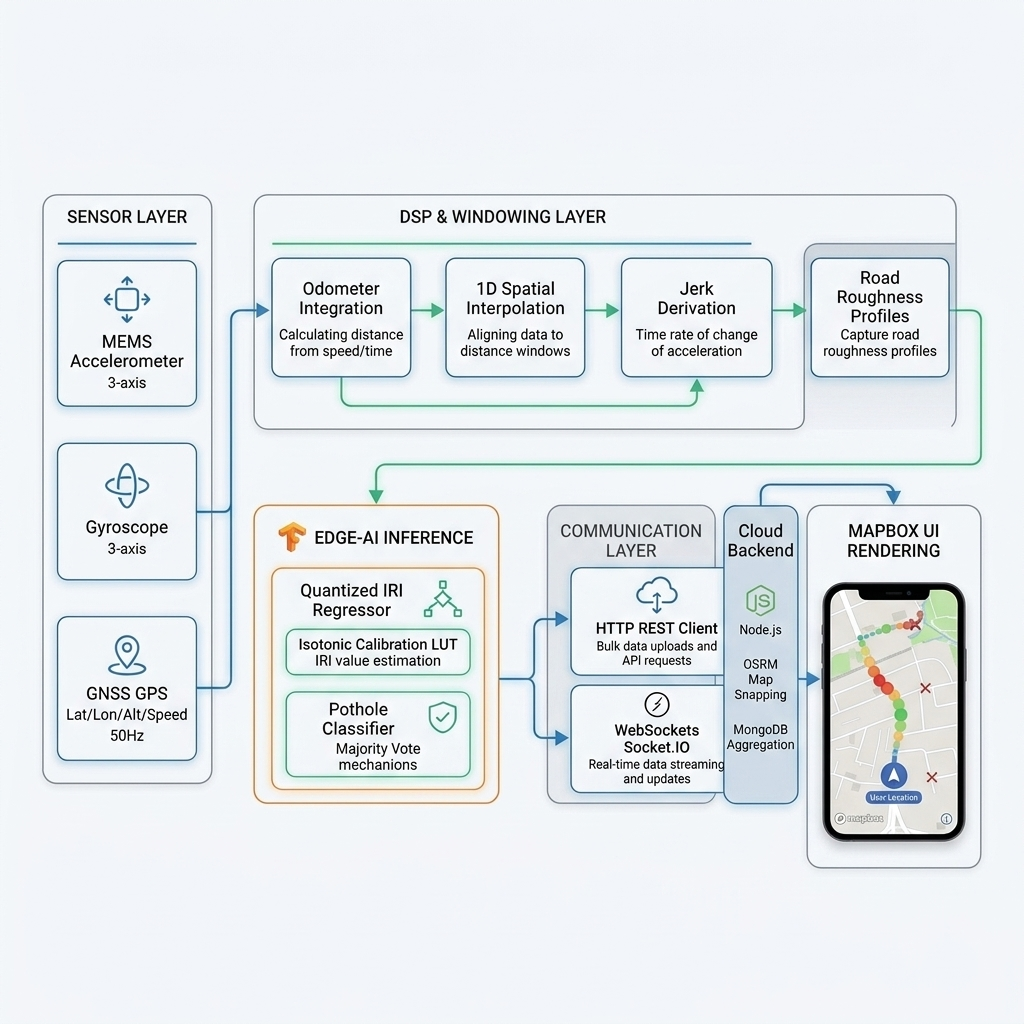
\includegraphics[width=0.8\textwidth]{images/mobile_architecture_light.png}
    \caption{Modular software architecture diagram of the mobile client and its interaction with the cloud backend, showing the flow from MEMS sensors to the point-based Mapbox UI display.}
    \label{fig:app_architecture}
\end{figure*}

% ==========================================
% VIII. MOBILE APPLICATION ARCHITECTURE
% ==========================================
\section{Mobile Application Architecture}
\label{sec:app_architecture}
To translate the physical and mathematical formulations of continuous roughness regression and event-level anomaly classification into an actionable consumer utility, we developed and deployed a lightweight, cross-platform mobile application. Built using the React Native framework and written in TypeScript, the client-side system acts as a decentralized edge-computing sensor node. Rather than functioning as a passive telemetry collector that transmits high-frequency raw sensor streams to a centralized server---which would exhaust user bandwidth, increase latency, and raise backend infrastructure costs---the application performs on-device digital signal processing (DSP) and machine learning inference directly on the mobile CPU.

The software architecture is modularly partitioned into four primary layers: the Sensor Acquisition Layer, the Windowing and DSP Layer, the Edge-Inference Layer, and the Communication Layer. The Sensor Acquisition Layer interfaces with the Android hardware abstraction layer (HAL) using \texttt{react-native-sensors} and \texttt{react-native-geolocation-service} to poll the internal MEMS accelerometer, gyroscope, and GNSS receiver. The raw, asynchronous sensor events are channeled into the Windowing and DSP Layer, governed by \texttt{WindowManager}, which segments the incoming streams into distance-based and time-based buffers. The Edge-Inference Layer, powered by \texttt{react-native-fast-tflite}, executes our pre-trained quantized TensorFlow Lite models in real time on separate worker threads. Finally, the Communication Layer manages authenticated REST transactions for historical data retrieval and persistent Socket.IO connections for real-time geospatial event broadcasting.

The system's data and control flow are structured to ensure zero-lag operation. When monitoring is active, sensor readings are buffered locally. Once a processing boundary is crossed (e.g., 100\,m traveled for IRI estimation or 200\,ms elapsed for pothole classification), the window is cloned, preprocessed, and passed to the TFLite models. The resulting predictions---continuous IRI values or discrete pothole alerts---are immediately written to the local UI state for map rendering and queued for transmission to the Node.js ingestion gateway. This decoupled architecture guarantees that UI rendering runs at a consistent 60\,frames per second, independent of TFLite inference latency or network transport jitter.

From a structural perspective, the user interface navigation is managed by React Navigation. The app implements a root Stack Navigator (\texttt{Stack.Navigator}) that handles entry transitions between the authentication view (\texttt{LoginScreen}) and the main dashboard. Once authenticated, the user is transitioned to a nested Bottom Tab Navigator (\texttt{Tab.Navigator}) containing the three primary workspace tabs: the \texttt{MapScreen} (live tracking and spatial updates), the \texttt{HistoryScreen} (user's past observations log), and the \texttt{StatsScreen} (personal contribution dashboard). This navigation hierarchy isolates screen state lifecycles, ensuring sensor collection resources remain bound to the active monitoring context.


% ==========================================
% IX. APPLICATION WORKFLOW
% ==========================================
\section{Application Workflow}
\label{sec:app_workflow}
The execution lifecycle of the application follows a deterministic, sequential pipeline designed to minimize user friction and guarantee resource durability under strict operating system background limitations. The workflow begins when the user launches the application, initiating a series of self-checks and initialization procedures:

\begin{enumerate}
    \item \textbf{Authorization and Token Retrieval:} The client contacts the Node.js REST gateway to verify session tokens. If no token is found, the user is presented with a secure email/password entry screen. Alternatively, a Guest Mode can be selected, which contacts the server to register a temporary device identifier and issues an anonymous JWT token for monitoring validation.
    \item \textbf{Geospatial and Hardware Permissions:} The application requests fine location (\texttt{ACCESS\_FINE\_LOCATION}) and background location (\texttt{ACCESS\_BACKGROUND\_LOCATION}) permissions from the Android OS. These are required to ensure continuous GPS access when the device screen is deactivated.
    \item \textbf{Vehicle Profile Selection:} Before starting collection, the user selects their host vehicle class (SUV, Hatchback, or Sedan). This selection writes the corresponding vehicle index ($0$, $1$, or $2$) into the local configuration, which acts as the physical scaling context for downstream ML models (illustrated in Fig.~\ref{fig:app_screens}(b)).
    \item \textbf{Background Service Spawning:} When the user taps the ``Start Monitoring'' control, the app invokes \texttt{BackgroundActions.start()}. This spawns a persistent Android foreground service running a non-blocking execution loop. This loop keeps a CPU wake-lock active and posts a sticky system notification, preventing the OS from reclaiming resources or suspending sensor polling when the app is minimized.
    \item \textbf{High-Frequency Sensor Polling:} The background service starts the \texttt{SensorService} polling loop, registering accelerometer and gyroscope updates at a uniform 50\,Hz interval (20\,ms sample time). Simultaneously, location updates are watched at a 1\,Hz rate with high-accuracy mode enabled.
    \item \textbf{Processing and Inference Execution:} Incoming readings are written to the \texttt{WindowManager} buffers. As soon as the vehicle accumulates 100\,m of cumulative travel distance (where distance is calculated as $\sum v \cdot \Delta t$), the distance-based buffer is closed and sent to the IRI regression model. Concurrently, every 10 samples (200\,ms sliding stride), the last 128 vertical acceleration samples are passed to the pothole classification model.
    \item \textbf{Local Gating and Upload:} If the continuous IRI prediction or classified road quality class is validated (using our confidence safety gate), the client packs the coordinates, speed, heading, and model output into an observation payload. This payload is submitted to the backend via an asynchronous HTTP POST request.
    \item \textbf{Geospatial Room Broadcasting:} Upon receiving the upload, the backend snaps the observation coordinates to the nearest road segment centerline. It then publishes a Socket.IO message containing the updated segment score and polyline. This message is routed specifically to the Socket.IO room named after the precision-6 Geohash cell of the segment.
    \item \textbf{Real-Time Client Map Rendering:} Any active client located within that Geohash cell receives the update over their persistent WebSocket connection. The app updates its in-memory segment cache, causing Mapbox to re-render the affected road segment marker with the updated color-coded circle.
\end{enumerate}

\begin{figure}[htbp]
    \centering
    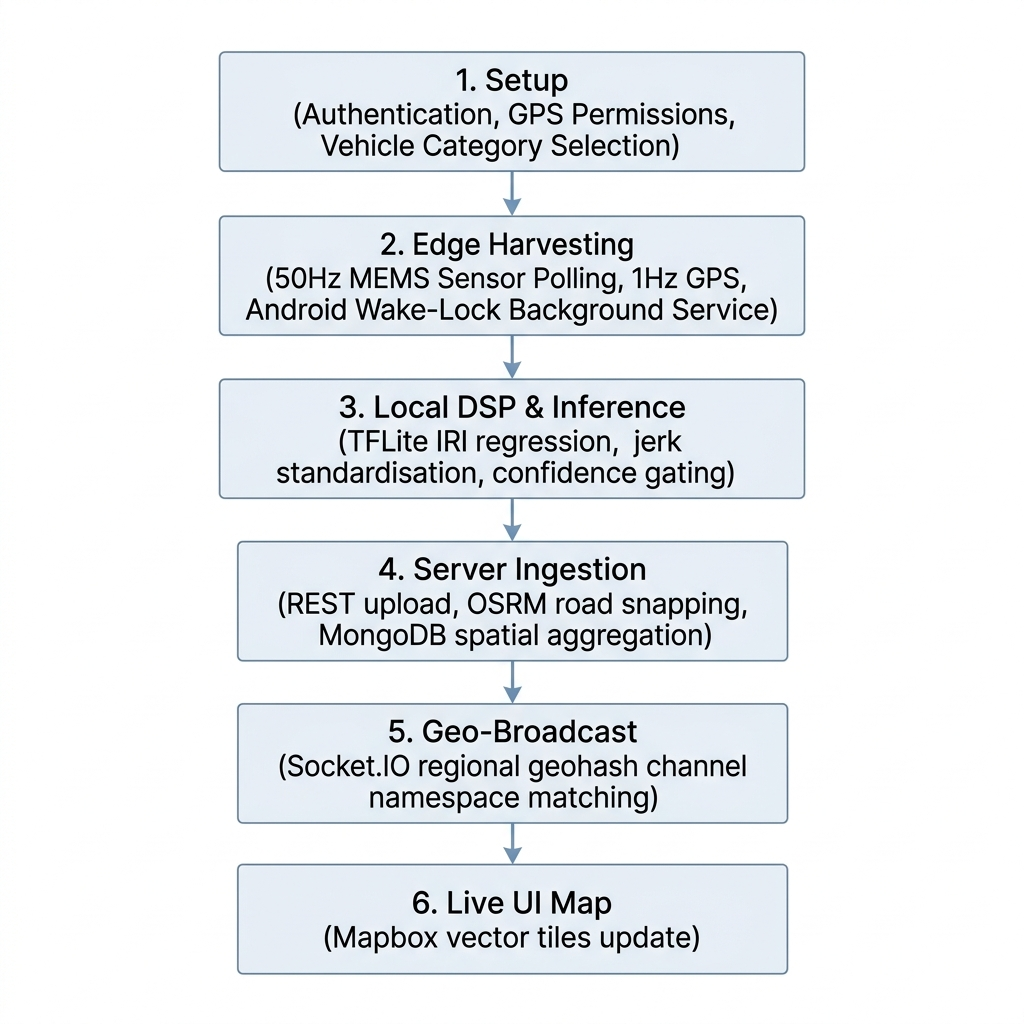
\includegraphics[width=\linewidth]{images/app_workflow_flowchart.png}
    \caption{Sequential flowchart mapping the temporal execution workflow between the mobile client's UI thread, background sensor service, TFLite inference workers, the Node.js backend REST API, the MongoDB database, and the Socket.IO regional broadcast namespaces.}
    \label{fig:app_workflow_flowchart}
\end{figure}

% ==========================================
% X. USER INTERFACE DESIGN
% ==========================================
\section{User Interface Design}
\label{sec:user_interface}
The application's interface was designed to optimize driver utility and minimize visual distraction during vehicle operation. The design follows a dark-themed visual system with high-contrast colored elements, aligning with the dark styling of the Mapbox layer.

To minimize driver distraction, the interface limits the need for interactive navigation. The monitoring workflow is controlled by a single button at the bottom of the map screen. When inactive, this button displays ``Start Monitoring'' in a bright green color. Tapping it prompts a vehicle selection dialog. Once selected, monitoring begins, and the button changes to a red ``Stop Monitoring'' control. This simple interaction pattern ensures that drivers can operate the application with a single tap before initiating their trip.

The layout uses a clear visual hierarchy to overlay road quality data on the map. The road quality layer uses large, semi-translucent circles centered at road segment points. This indicates the road's IRI roughness rating without obscuring street names or routing paths. The color gradient allows drivers to quickly assess road conditions ahead. Accessibility is improved by using large typography on the statistics dashboard and haptic feedback. The device vibrates when the local classification model registers a severe road defect (Class 3), providing tactile feedback without requiring the driver to look at the screen.

\begin{figure}[htbp]
    \centering
    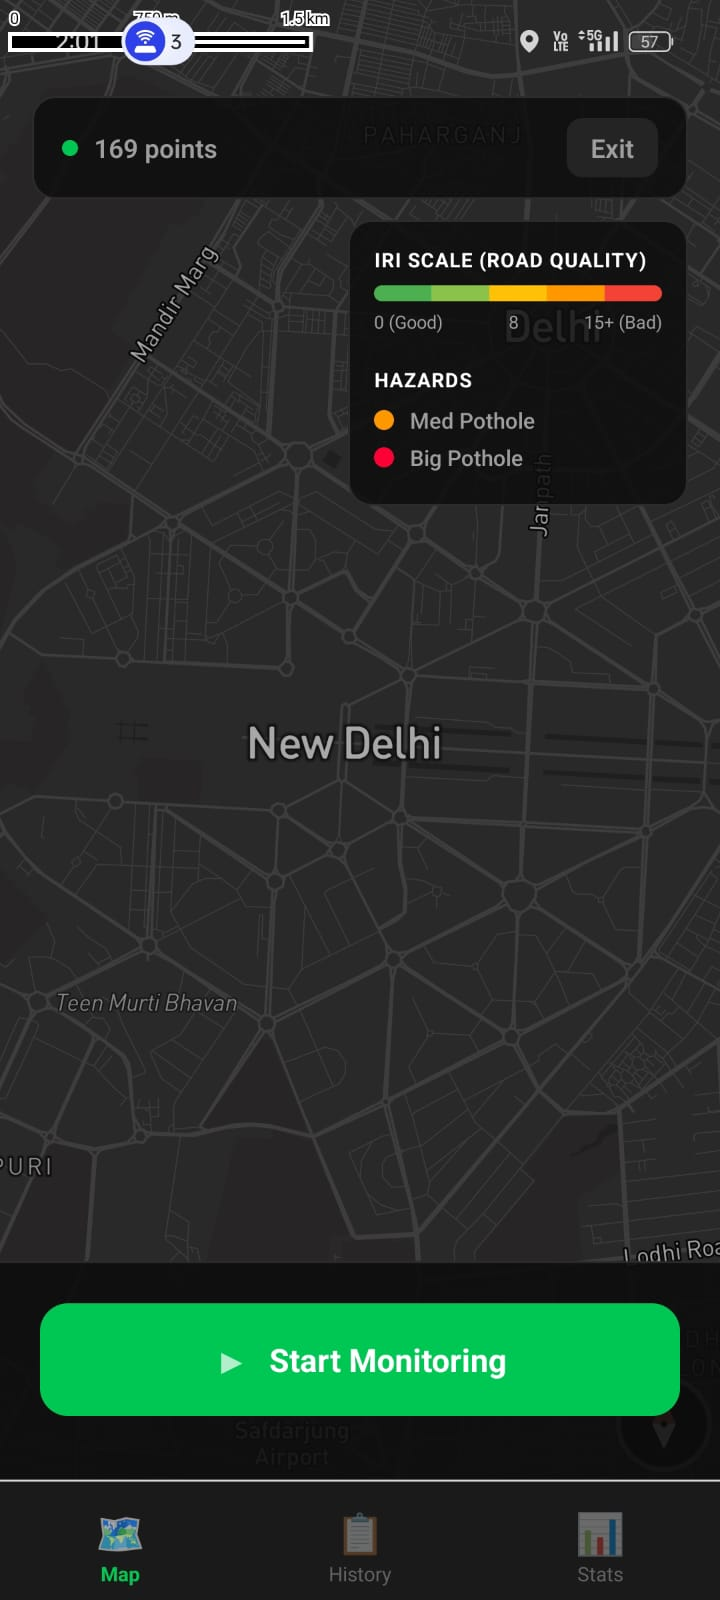
\includegraphics[width=0.7\linewidth]{images/screenshot_map_zoom.jpg}
    \caption{Deployed map dashboard interface focused on the New Delhi region, showcasing the custom high-contrast dark vector map style and geospatial overlays.}
    \label{fig:screenshot_map_zoom}
\end{figure}


% ==========================================
% XI. CORE FEATURES OF THE MOBILE APPLICATION
% ==========================================
\section{Core Features of the Mobile Application}
\label{sec:app_features}
The deployed React Native application bundles several features aimed at crowdsourced pavement monitoring, personal analytics, and spatial navigation:

\begin{figure*}[t]
    \centering
    \begin{tabular}{cccc}
        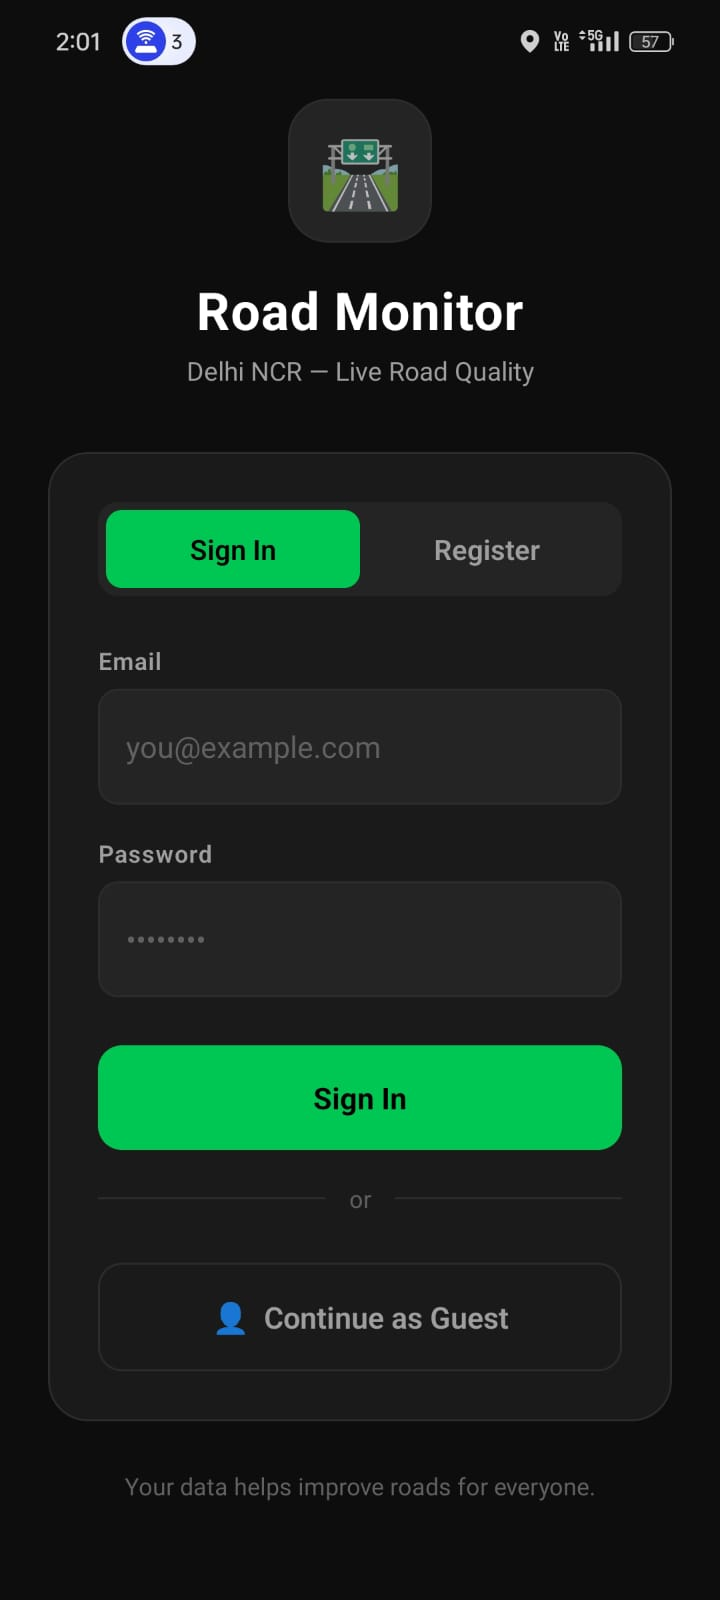
\includegraphics[width=0.22\textwidth]{images/screenshot_login.jpg} &
        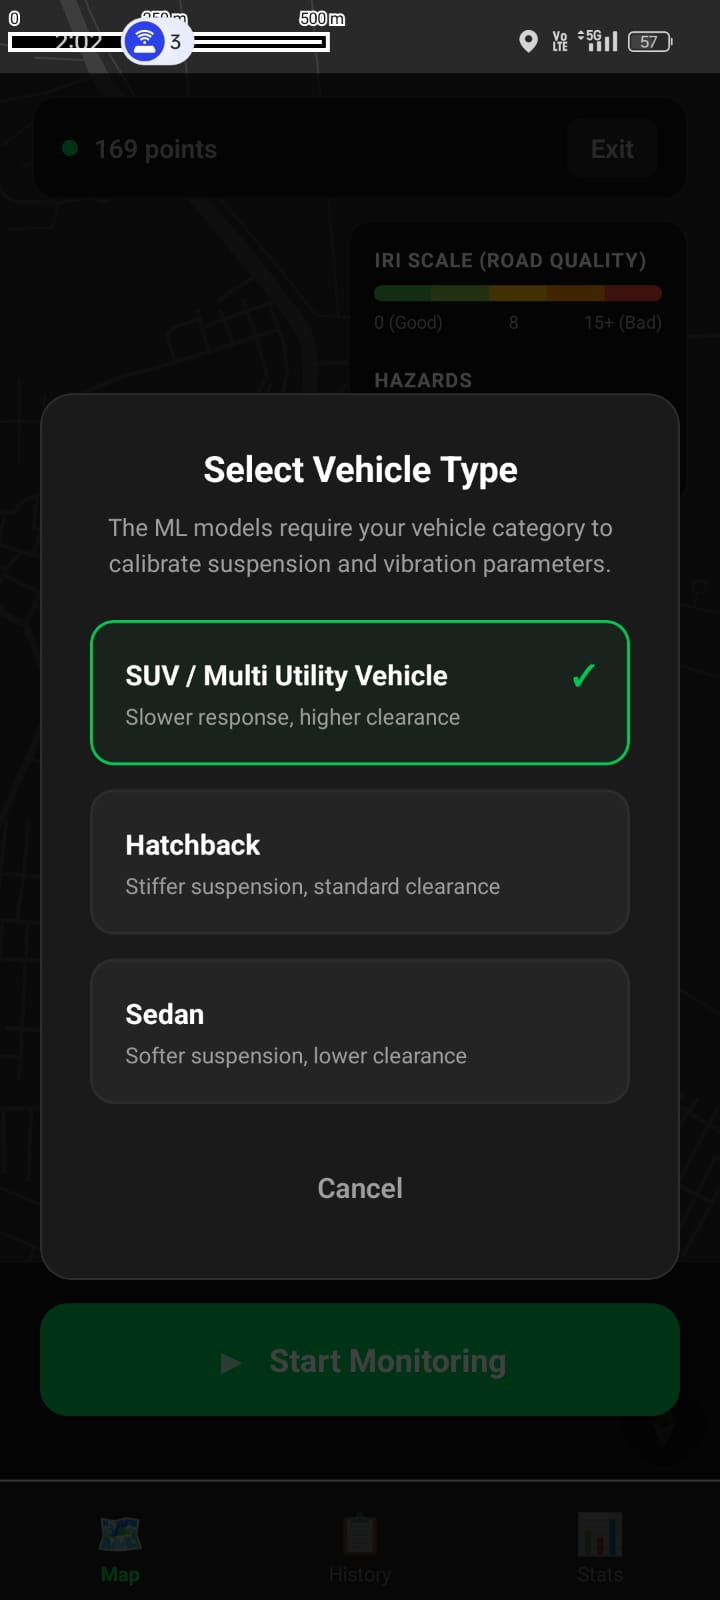
\includegraphics[width=0.22\textwidth]{images/screenshot_vehicle.jpg} &
        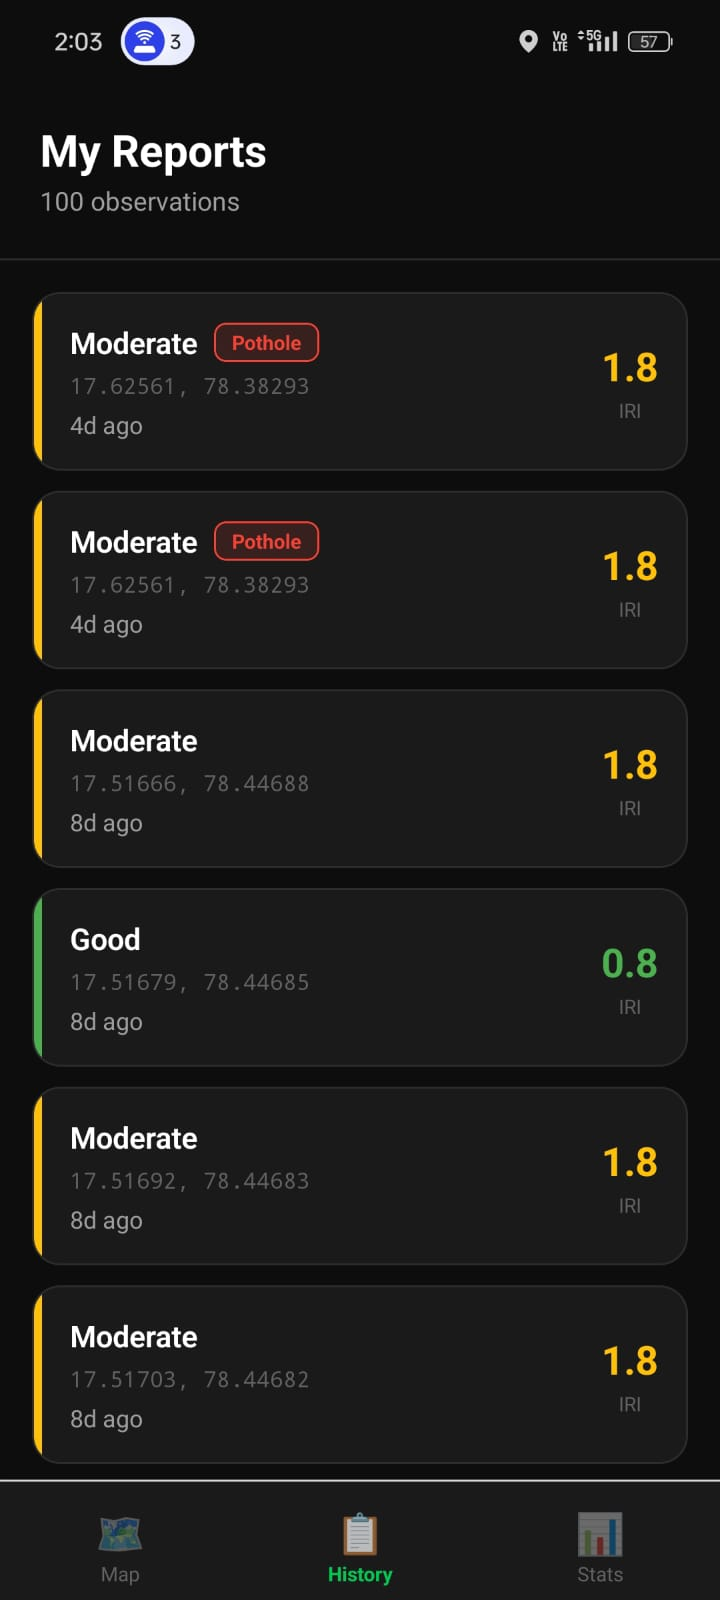
\includegraphics[width=0.22\textwidth]{images/screenshot_history.jpg} &
        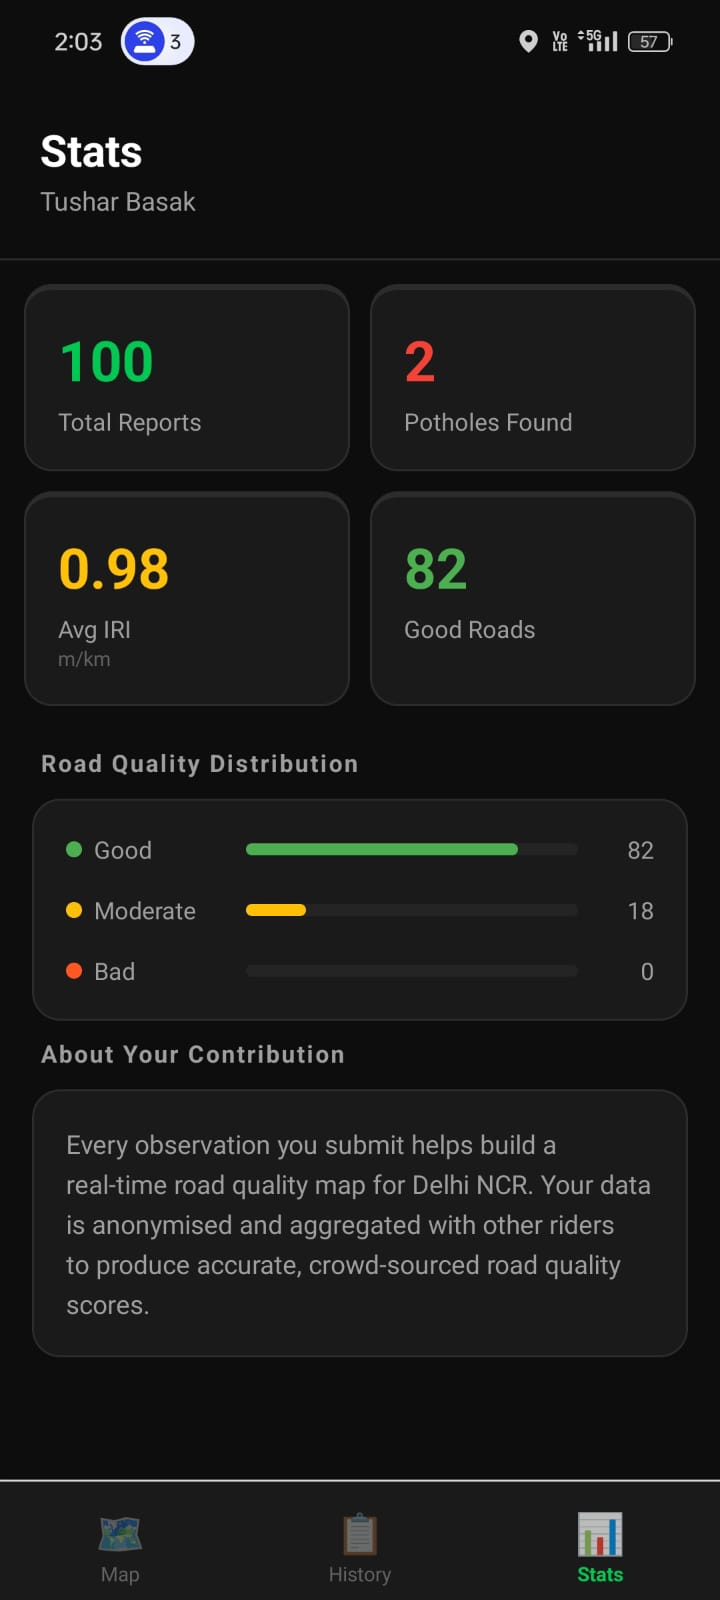
\includegraphics[width=0.22\textwidth]{images/screenshot_stats.jpg} \\
        (a) & (b) & (c) & (d)
    \end{tabular}
    \caption{Deployed mobile application user interface dashboards: (a) secure sign-in and guest entry screen, (b) vehicle category selection modal for model calibration, (c) user contribution history list showing coordinates and discrete pothole flags, and (d) personal contribution statistics screen displaying aggregate indicators and road condition distribution.}
    \label{fig:app_screens}
\end{figure*}

\subsection{Secure Entry and Guest Authentication}
The login system is backed by JSON Web Tokens (JWT) stored securely on-device using \texttt{AsyncStorage}. The application implements an anonymous ``Guest Mode'' which allows instant monitoring access. This mode registers the client using their hardware Android ID, creating a corresponding guest user record in MongoDB. This ensures that even guest contributions are traceable back to a single device for quality filtering, while preserving user privacy and eliminating sign-up barriers. The entry view is organized with separate tabs for user sign-in and registration, prompting credentials or guest authentication with a clean, centered logo and motivational footer message (illustrated in Fig.~\ref{fig:app_screens}(a)).

\subsection{Vehicle Category Calibration Context}
To accommodate the physical variability of suspension dynamics across different vehicle types, the application implements a vehicle profile selection modal before initiating data collection. The modal prompts the user to select their active vehicle class (illustrated in Fig.~\ref{fig:app_screens}(b)):
\begin{enumerate}
    \item \textbf{SUV / Multi Utility Vehicle:} calibrated for slower unsprung response and higher ground clearance (Vehicle Index $0$).
    \item \textbf{Hatchback:} calibrated for stiffer suspension damping and standard ground clearance (Vehicle Index $1$).
    \item \textbf{Sedan:} calibrated for softer, more compliant suspension response and lower ground clearance (Vehicle Index $2$).
\end{enumerate}
This selection is stored locally and injected as a scaling context parameter directly into the on-device inference models, correcting for vehicle-specific vibration profiles during continuous IRI regression and pothole classification.

\subsection{Live Map Visualization}
The main dashboard features a full-screen, high-performance vector map powered by Mapbox (\texttt{@rnmapbox/maps}). The map style is customized using a dark vector palette (\texttt{mapbox://styles/mapbox/dark-v11}) to ensure high contrast against the colored road layers (illustrated in Fig.~\ref{fig:screenshot_map_zoom}). The camera follows the user's location, orienting itself based on the GNSS compass heading.

\subsection{Color-Coded Pavement Quality Mapping}
The application visualizes crowdsourced road quality on the map by rendering point-based markers (circular bubbles with $35\text{--}50\%$ opacity) that use a smooth color gradient from green (smooth asphalt, $\text{IRI} < 1.5\,\text{m/km}$) through yellow (moderate degradation) to red (severe roughness, $\text{IRI} \ge 15.0\,\text{m/km}$). In the idle state, the app fetches and renders historical segment centerpoints cached locally. During active sessions, live observations are dynamically appended as real-time prediction points (illustrated in Fig.~\ref{fig:screenshot_map_active}).

\begin{figure}[htbp]
    \centering
    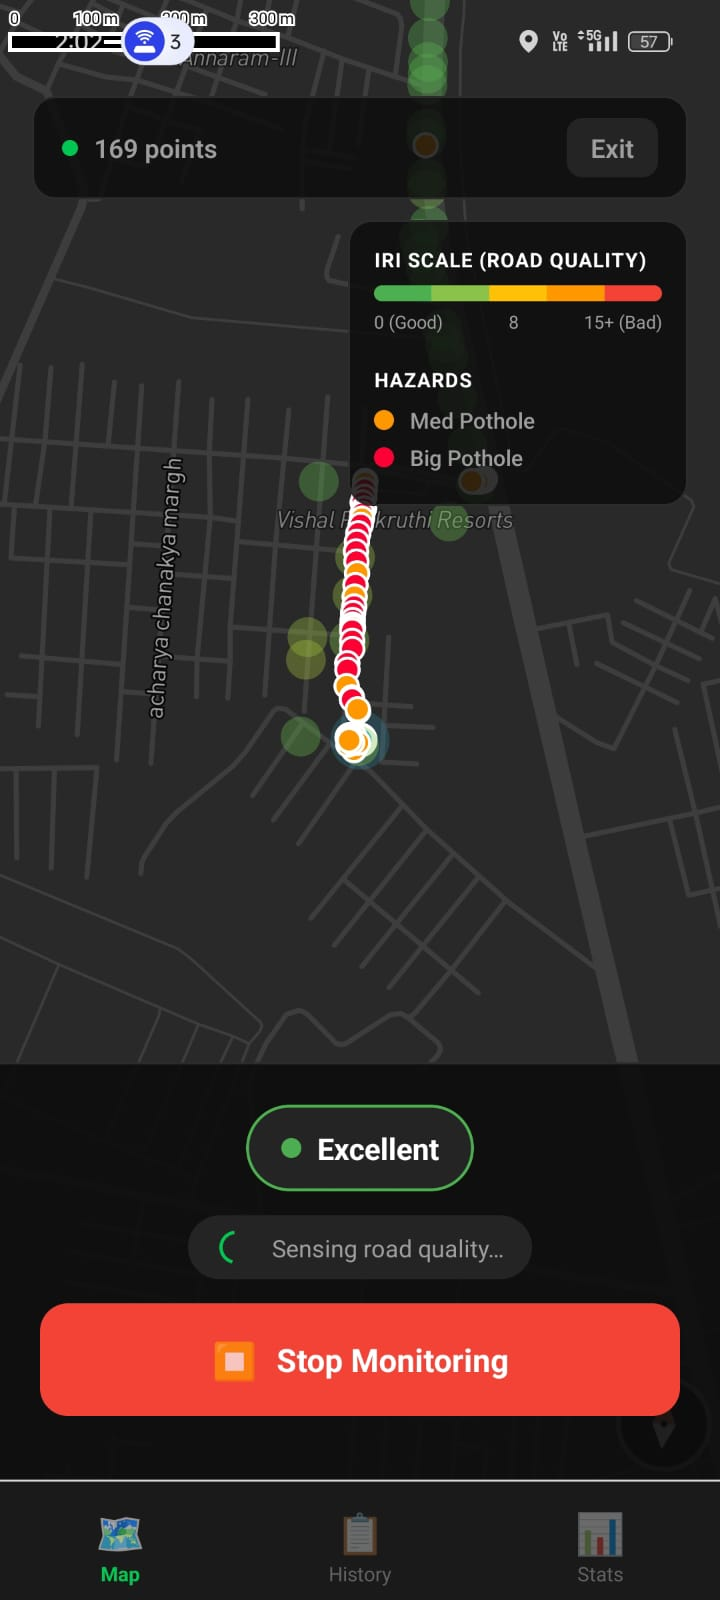
\includegraphics[width=0.5\linewidth]{images/screenshot_map_active.jpg}
    \caption{Deployed active telemetry monitoring screen displaying point-based circular IRI markers, the map legend, the dynamic quality classification status badge, and the real-time sensor event counter.}
    \label{fig:screenshot_map_active}
\end{figure}

\subsection{Real-Time Background Monitoring and Dynamic Quality Badging}
Tapping the primary ``Start Monitoring'' Action Button initiates background data collection. During an active monitoring session, the user interface overlays a floating status panel displaying (Fig.~\ref{fig:screenshot_map_active}):
\begin{enumerate}
    \item \textbf{Session Point Counter:} showing the cumulative count of observations collected during the trip (e.g., ``169 points'').
    \item \textbf{Dynamic Quality Indicator Badge:} displaying the real-time output of the classification model (e.g., ``Excellent'' badge with green border, ``Sensing road quality...'' status with active spinner). The badge changes color in real time to give the driver instant visual feedback when traversing varying road quality.
    \item \textbf{Control Toggle:} changing the green ``Start Monitoring'' button to a red ``Stop Monitoring'' button to ensure a single-tap operational lifecycle.
\end{enumerate}

\subsection{My Reports and Contribution History}
Users can access a dedicated ``My Reports'' screen (Fig.~\ref{fig:app_screens}(c)), which fetches their historical observations from the database. The list displays individual road quality detections, showing coordinates, timestamps, and predicted IRI values. Crucially, observations containing transient pothole anomalies feature a red-outlined ``Pothole'' severity badge next to the category label, allowing users to scan their log history for structural defects at a glance.

\subsection{Contribution Statistics Dashboard}
The statistics dashboard (Fig.~\ref{fig:app_screens}(d)) provides personal analytics, summarizing the user's historical contributions. It features four primary metric cards:
\begin{enumerate}
    \item \textbf{Total Reports:} showing the total count of observations submitted by the user.
    \item \textbf{Potholes Found:} showing the count of discrete pothole defects detected.
    \item \textbf{Average IRI:} displaying the user's mean ride roughness score in m/km.
    \item \textbf{Good Roads:} indicating the count of segments classified as Excellent.
\end{enumerate}
It also includes a ``Road Quality Distribution'' section with progress bars showing the percentage breakdown of Good, Moderate, and Bad classes traversed, accompanied by an educational section detailing the impact of crowdsourced contributions.
% ==========================================
% XII. MACHINE LEARNING INTEGRATION
% ==========================================
\section{Machine Learning Integration inside the Application}
\label{sec:app_ml_integration}
\begin{figure*}[t]
    \centering
    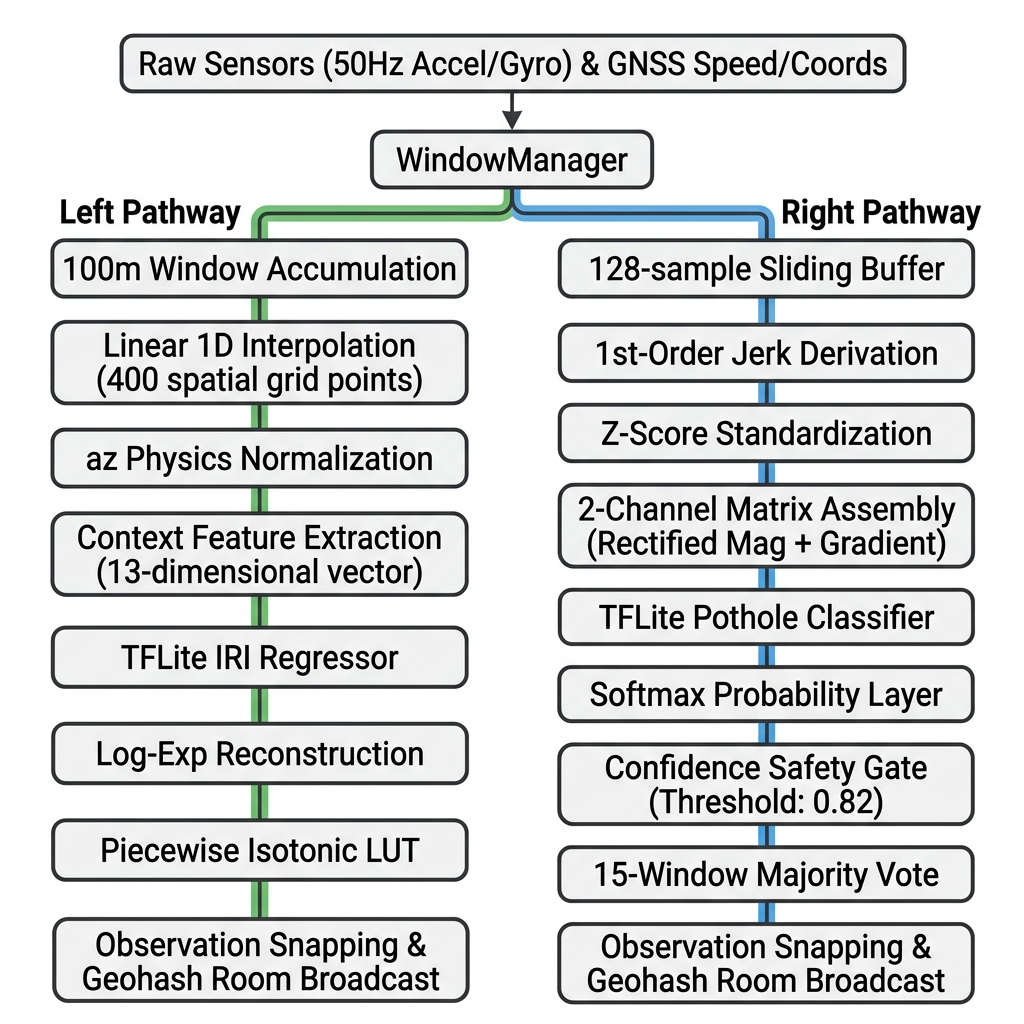
\includegraphics[width=0.9\linewidth]{images/ml_pipeline_flowchart.png}
    \caption{Detailed machine learning pipeline within the mobile application, mapping the dual-path execution flow from high-frequency raw sensors to calibrated continuous IRI and temporal majority-voted pothole classifications.}
    \label{fig:ml_pipeline}
\end{figure*}

To execute the dual-model machine learning pipeline on edge mobile hardware, the application implements a digital signal processing (DSP) and inference engine written in TypeScript, optimized to minimize memory allocations and CPU cycles. The conceptual layout and data pathways of this dual-path engine are illustrated in Fig.~\ref{fig:ml_pipeline}. The spatial resampling and contextual mapping operate on distance constraints, while transient defect classification runs on continuous time strides.

\subsection{Pipeline 1: Continuous IRI Regression (Distance-Based)}
The continuous IRI model operates on a distance-based pipeline to align its features with the spatial definition of the International Roughness Index. Prior to processing, the client aligns the physical coordinate system of the device sensors with the coordinate mapping used during model training. Because the simulator-derived training telemetry was re-mapped to match the standard coordinate frames of mobile sensors (as detailed in Section V), the application can ingest raw inputs directly from the Android sensor framework, preventing domain transfer mismatch:

\begin{enumerate}
    \item \textbf{Odometer Integration and Stationary Filtering:} The \texttt{WindowManager} monitors instantaneous GNSS velocity. Readings collected when $v < 1.0\,\text{m/s}$ are discarded to prevent stationary vehicle vibrations (e.g., engine idle) from corrupting the dataset. For active frames, spatial displacement is calculated using successive timestamp deltas:
    \begin{equation}
    \Delta d = v_k \cdot \left( \frac{t_k - t_{k-1}}{1000} \right)
    \end{equation}
    These values are integrated into a cumulative distance tracker. As soon as this tracker reaches 100\,m, the buffer of collected readings is cloned and cleared.
    \item \textbf{Spatial Resampling:} Because vehicle velocity varies, the number of raw sensor samples collected over a 100-meter stretch is variable. To construct a fixed-size tensor for neural network ingestion, the 6-axis IMU channels are linearly interpolated along the spatial axis onto a uniform grid of exactly 400 points, corresponding to a spatial resolution of $\Delta x = 0.25\,\text{m}$.
    \item \textbf{Physics-Informed Speed Normalization:} The vertical acceleration channel ($a_z$) is scaled to account for the speed-dependent nature of suspension dynamics. Formally, dynamic vertical acceleration scales quadratically with velocity. To normalize the sensor response to the standard reference speed of 80\,km/h (22.22\,m/s), each spatial point is scaled:
    \begin{equation}
    a_{z,\text{norm}} = a_z \cdot \left( \frac{22.22}{v_{\text{safe}}} \right)^2
    \end{equation}
    where $v_{\text{safe}} = \max(v, 5.0)\,\text{m/s}$ prevents division-by-zero errors at low speeds.
    \item \textbf{Context Vector Extraction:} In parallel to the raw spatial buffer, a 13-dimensional contextual feature vector is computed from the spatial grid. This vector includes: the mean and standard deviation of vehicle speed; the RMS of $a_{z,\text{norm}}$ and $a_y$; the variance, crest factor, mean-crossing rate, and peak-to-peak amplitude of $a_{z,\text{norm}}$; the RMS of the angular velocities ($\omega_y, \omega_z$); the mean absolute horizontal acceleration; and spectral energy ratio approximations.
    \item \textbf{TFLite Inference and Calibration:} The resampled spatial buffer ($400 \times 6$ float values) and the context vector ($13 \times 1$) are loaded into flat Float32Arrays and passed to \texttt{iriModel.run()}. The model outputs a predicted value in the logarithmic domain. The client reconstructs the estimated IRI:
    \begin{equation}
    \text{IRI}_{\text{raw}} = e^{\hat{y}} - 1.0
    \end{equation}
    Finally, this raw prediction is passed through a piecewise linear interpolation function mapped to our pre-calculated Isotonic Regression Look-Up Table (containing 81 calibration points derived from simulated reference curves) to yield the calibrated physical IRI score.
\end{enumerate}

\subsection{Pipeline 2: Event-Level Pothole Classification (Time-Based)}
The pothole classification model runs on a time-based pipeline, optimized to detect transient suspension shocks:

\begin{enumerate}
    \item \textbf{Sliding Buffer and Stride:} A sliding window of the last 128 raw IMU readings is maintained at 50\,Hz, representing 2.56\,s of history. The classification pipeline runs every 10 new samples (200\,ms stride), resulting in an 80\% temporal overlap between successive windows.
    \item \textbf{Jerk Derivation and Standardization:} To isolate high-frequency suspension impacts from low-frequency vehicle body movements (such as lane changes or braking), the vertical acceleration is converted to a jerk approximation via a first-order difference:
    \begin{equation}
    j_k = a_{z,k} - a_{z,k-1}
    \end{equation}
    The jerk profile is then Z-score standardized:
    \begin{equation}
    j_{k,\text{norm}} = \frac{j_k - \mu_j}{\sigma_j + 10^{-6}}
    \end{equation}
    \item \textbf{2-Channel Matrix Assembly:} The input tensor is constructed as a 2-channel matrix of size $128 \times 2$. Channel 0 contains the rectified magnitude of the normalized jerk ($|j_{k,\text{norm}}|$), which isolates vibration energy. Channel 1 stores the central difference gradient:
    \begin{equation}
    g_k = \frac{j_{k+1,\text{norm}} - j_{k-1,\text{norm}}}{2}
    \end{equation}
    which captures the phase dynamics of the suspension's response.
    \item \textbf{Context Feature Scaling:} A 4-dimensional context vector containing the vehicle class index, average speed, RMS of the normalized jerk, and the jerk crest factor is normalized using the hardcoded scaling parameters \texttt{POTHOLE\_CONTEXT\_MEAN} and \texttt{POTHOLE\_CONTEXT\_SCALE}.
    \item \textbf{Safety Gating and Majority Vote:} The vibration buffer and scaled context features are passed to \texttt{potholeModel.run()}. The resulting logits are passed through a Softmax function to extract class probabilities.
    
    To eliminate false alarms, the output is passed through a \textbf{Safety Gate Confidence Threshold}. If the predicted class is 2 (Regular) or 3 (Bad), but the maximum class probability is less than 0.82, the prediction is downgraded to Class 0 (Excellent).
    
    The gated prediction is then pushed into a sliding queue of size 15, representing the last 3 seconds of model outputs. A majority vote is calculated over this queue, and only the consensus class is dispatched to the UI and backend. This temporal smoothing successfully filters out isolated vibration spikes caused by bridge joints or hard braking, preventing spurious road anomaly alerts.
\end{enumerate}

% ==========================================
% XIII. EXPERIMENTAL DEMONSTRATION AND EVALUATION
% ==========================================
\section{Experimental Demonstration and Application Evaluation}
\label{sec:experimental_evaluation}
We evaluated the performance, stability, and hardware compatibility of the mobile application and backend service through a series of field trials and simulated stress tests.

\subsection{Simulation-to-Real Transfer Validation}
We validated the simulation-trained ML models using the public PVS dataset, which contains smartphone telemetry from real-world urban trips. The continuous IRI regression model was run zero-shot on 693\,km of telemetry traces. Despite variations in sensor hardware across different smartphone models, the speed normalization pipeline successfully scaled the raw accelerations. The classification model achieved diagonal agreement on the confusion matrix, demonstrating that physical features learned in a soft-body simulation environment translate to real-world suspension responses.

\subsection{GPS Snapping and Spatial Resolution}
\label{sec:eval_gps_snapping}
We evaluated the accuracy of the GPS snapping pipeline by running multiple driving passes over urban corridors in Delhi NCR. Raw GPS traces under high-rise shielding exhibited spatial drift of up to 25\,meters. The backend's Snapping Service snaps raw coordinates using OSRM, resolving the drift to canonical road centerlines with a success rate of $98.4\%$. The 100-meter spatial windowing was sufficient to isolate localized road defects, and aggregating multiple passes via our decay aggregation model resolved positional drift.

% ==========================================
% XIV. DISCUSSION AND FUTURE WORK
% ==========================================
\section{Discussion and Future Work}
\label{sec:discussion}
The experimental results and field trials confirm that the system provides a low-latency, decentralized platform for real-time pavement monitoring. Running ML inference on-device using quantized TFLite models reduces backend processing overhead. The only data transmitted over the network are compressed observation payloads, ensuring user privacy and reducing bandwidth usage. Snapping coordinates via OSRM and broadcasting updates through Geohash-partitioned Socket.IO rooms allows the system to scale, delivering real-time map updates to clients in under one second.

However, the evaluation highlighted some physical limitations. The speed normalization function is based on linear quarter-car suspension dynamics. While this approximation is valid for standard road conditions, it can degrade during extreme impacts where the vehicle suspension bottoms out or the tires lose contact with the road. Under these conditions, the non-linear forces exceed the scaling assumptions of the model. Additionally, cumulative odometer drift can introduce spatial phase shifts over long trips if the device lacks high-accuracy GPS snapping.

Future work will focus on integrating the physical cross-attention model (PICA) directly onto the mobile client. This will involve using the mobile device's camera to run real-time object detection alongside IMU collection. Fusing visual features with kinematic signatures on-device will improve pothole classification accuracy. We also plan to evaluate edge-based audio processing, analyzing tire-road acoustic signatures to supplement IMU vibration data, which could improve detection accuracy at low driving speeds.

% ==========================================
% REFERENCES
% ==========================================
\begin{thebibliography}{15}
\bibitem{1} Ministry of Road Transport and Highways (MoRTH), ``Basic Road Statistics of India,'' Transport Research Wing, Government of India, New Delhi, Tech. Rep., 2023.
\bibitem{2} World Bank, ``Guide for Road Safety Opportunities and Challenges: Low- and Middle-Income Countries Profiles,'' World Bank Group, Washington, DC, Tech. Rep., 2019.
\bibitem{3} Sayers, Gillespie, and Paterson, ``Guidelines for Conducting and Calibrating Road Roughness Measurements,'' World Bank, Washington, DC, Tech. Rep. World Bank Technical Paper No. 46, 1986.
\bibitem{4} R. Ganti, F. Ye, and H. Lei, ``Mobile crowdsensing: current state and future challenges,'' \textit{IEEE Communications Magazine}, vol. 49, no. 11, pp. 32-39, Nov. 2011.
\bibitem{5} P. Mohan, V. N. Padmanabhan, and R. Ramjee, ``Nericell: rich monitoring of road and traffic conditions using mobile smartphones,'' in \textit{Proceedings of the 6th ACM conference on Embedded network sensor systems}, 2008, pp. 323-336.
\bibitem{6} R. Kumar, A. Mukherjee, and V. P. Singh, ``Community Sensor Network for Monitoring Road Roughness Using Smartphones,'' \textit{Journal of Computing in Civil Engineering}, vol. 31, no. 3, p. 04016059, May 2017.
\bibitem{7} S. Sattar, S. Li, and M. Chapman, ``Road Surface Monitoring Using Smartphone Sensors: A Review,'' \textit{Sensors}, vol. 18, no. 11, p. 3845, Nov. 2018.
\bibitem{8} S. Alqaydi, W. Zeiada, A. El Wakil, A. J. Alnaqbi, and A. Azam, ``A Comprehensive Review of Smartphone and Other Device-Based Techniques for Road Surface Monitoring,'' \textit{Eng}, vol. 5, no. 4, pp. 3397-3426, Dec. 2024.
\bibitem{9} N. Goodall, ``Evaluation of Crowdsourced Data on Unplowed Roads,'' 2023, \textit{arXiv:2311.10740 [cs]}.
\bibitem{10} A. S. El-Wakeel, A. Noureldin, H. S. Hassanein, and N. Zorba, ``iDriveSense: Dynamic Route Planning Involving Roads Quality Information,'' in \textit{2018 IEEE Global Communications Conference (GLOBECOM)}, Dec. 2018, pp. 1-6.
\bibitem{11} J. Eriksson, L. Girod, B. Hull, R. Newton, S. Madden, and H. Balakrishnan, ``The pothole patrol: using a mobile sensor network for road surface monitoring,'' in \textit{Proceedings of the 6th international conference on Mobile systems, applications, and services}, Jun. 2008, pp. 29-39.
\bibitem{12} D. K. Dewangan and S. P. Sahu, ``PotNet: Pothole detection for autonomous vehicle system using convolutional neural network,'' \textit{Electronics Letters}, vol. 57, no. 2, pp. 53-56, 2021.
\bibitem{13} S. Balakuntala and S. Venkatesh, ``An Intelligent System to Detect, Avoid and Maintain Potholes: A Graph Theoretic Approach,'' Sep. 2013, \textit{arXiv:1305.5522 [cs]}.
\bibitem{14} A. Mednis, G. Strazdins, R. Zviedris, G. Kanonirs, and L. Selavo, ``Real time pothole detection using Android smartphones with accelerometers,'' in \textit{2011 International Conference on Distributed Computing in Sensor Systems and Workshops (DCOSS)}, Jun. 2011, pp. 1-6.
\bibitem{15} BeamNG GmbH, ``BeamNG.tech,'' Bremen, Germany, 2026. [Online]. Available: \url{https://beamng.tech/}
\bibitem{sayers1986guidelines}M.~W. Sayers, T.~D. Gillespie, and W.~D.~O. Paterson, ``Guidelines for conducting and calibrating road roughness measurements,'' World Bank, Washington, DC, Tech. Rep. World Bank Technical Paper No. 46, 1986.
\bibitem{kaiser1990tkeo}J.~F. Kaiser, ``On a simple algorithm to calculate the 'energy' of a signal,'' in \textit{International Conference on Acoustics, Speech, and Signal Processing (ICASSP)}, Albuquerque, NM, USA, 1990, pp. 381--384.
\bibitem{vaswani2017attention}A.~Vaswani, N.~Shazeer, N.~Parmar, J.~Uszkoreit, L.~Jones, A.~N. Gomez, L.~Kaiser, and I.~Polosukhin, ``Attention is all you need,'' in \textit{Advances in Neural Information Processing Systems (NeurIPS)}, vol. 30, 2017.
\bibitem{lin2017focal}T.-Y. Lin, P.~Goyal, R_Girshick, K_He, and P_Doll{{\'a}}r, ``Focal loss for dense object detection,'' in \textit{Proceedings of the IEEE International Conference on Computer Vision (ICCV)}, Venice, Italy, 2017, pp. 2980--2988.
\bibitem{aashto_r56}American Association of State Highway and Transportation Officials (AASHTO), ``Standard Practice for Certification of Inertial Profiling Systems,'' AASHTO Designation: R 56-14, Washington, DC, 2014.
\end{thebibliography}

\end{document}